\chapter{Resultados}
\label{resultados}



\section{Pré Diagnóstico e Sócio Tecnológico}
\label{pre_diagnostico_socio_tec}

No total, participaram oito docentes do universo populacional pesquisado, sendo 37,5\% mulheres e 62,5\% homens, conforme ilustrado na Figura \ref{fig:genero_participantes}. Embora tenha ocorrido um aumento no ingresso de mulheres no ensino superior, sua presença nos cursos de matemática e estatística permanece reduzida. Essa realidade é destacada em um boletim divulgado em 12 de maio de 2023 pela Sociedade Brasileira de Matemática (SBM) e pela Sociedade Brasileira de Matemática Aplicada e Computacional (SBMac), em colaboração com a Associação Brasileira de Estatística, que reforça a sub-representação feminina nessas áreas.

\begin{figure}[h!]
    \caption{Gênero dos Participantes}
    \centering
    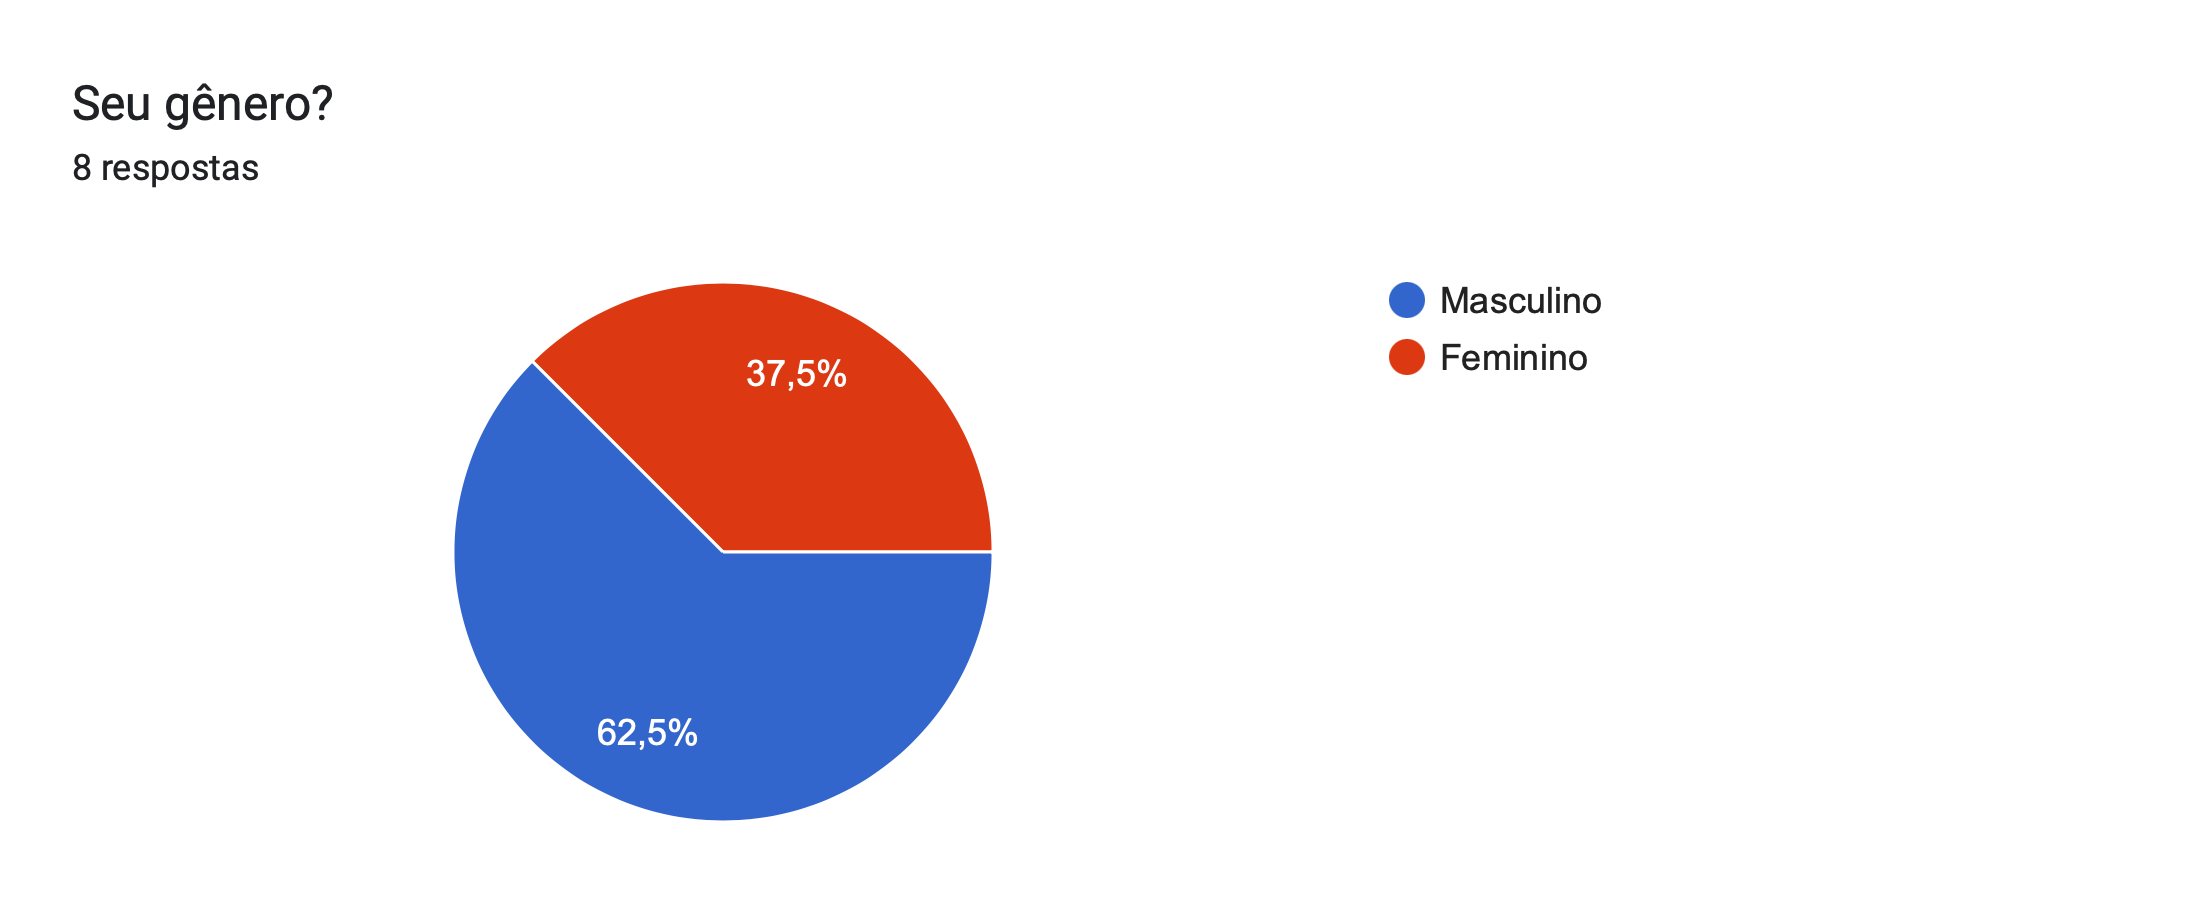
\includegraphics[scale=0.2]{figuras/resultados/genero.png}
    \label{fig:genero_participantes}
    \legend{Fonte: Eonay e Klenilmar (2024).}
\end{figure}

A participação das mulheres nas ciências exatas, embora crescente, ainda enfrenta desafios significativos, especialmente em áreas como matemática, estatística e física. Estudos indicam que fatores históricos, culturais e sociais têm contribuído para a sub-representação feminina nesses campos, perpetuando estereótipos de gênero que desencorajam sua inserção. Segundo um levantamento da \cite{brasil2018decifrar}, as mulheres representam apenas cerca de 30\% dos pesquisadores em áreas STEM (Ciência, Tecnologia, Engenharia e Matemática) no mundo.

No Brasil, conforme aponta o boletim da Sociedade Brasileira de Matemática (SBM) e da Sociedade Brasileira de Matemática Aplicada e Computacional (SBMac) de 2023, a disparidade é evidente nos cursos de matemática e estatística, que continuam sendo predominantemente masculinos. Promover iniciativas de inclusão e destacar modelos femininos de sucesso são estratégias fundamentais para equilibrar essa desigualdade e estimular novas gerações de mulheres a ingressarem e se destacarem nas ciências exatas.



Um aspecto analisado no estudo foi a experiência docente relacionada ao ensino do conteúdo de matrizes, uma estrutura amplamente utilizada em diversas disciplinas e áreas do conhecimento. Os dados revelam que 62,5\% dos participantes afirmaram já ter trabalhado diretamente com o tema, enquanto 37,5\% indicaram ainda não tê-lo abordado, como ilustrado na Figura \ref{fig:trabalhou_matrizes}. O uso de matrizes é essencial em áreas como matemática aplicada, estatística e ciência de dados, destacando sua relevância na formação acadêmica e interdisciplinar \cite{golub2013matrix}.

\begin{figure}[h!]
    \caption{Trabalhou diretamente com o conteúdo de Matrizes}
    \centering
    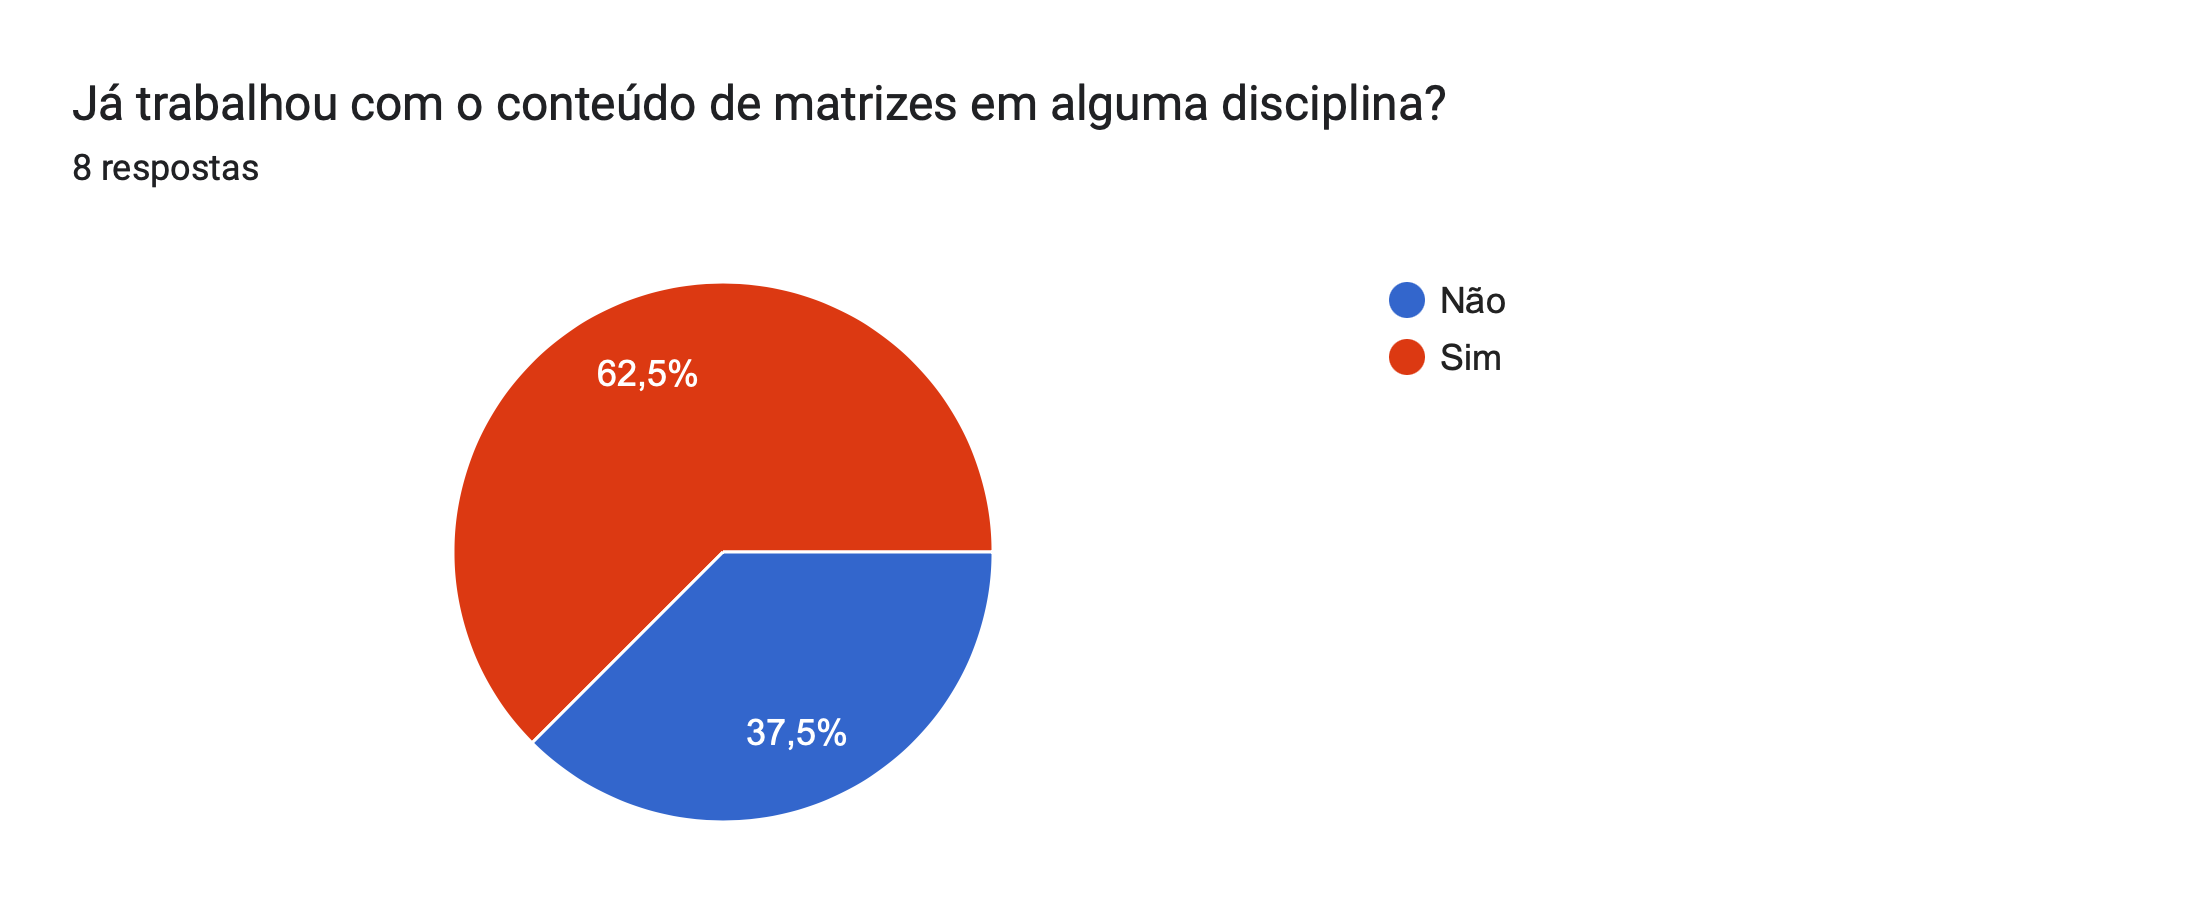
\includegraphics[scale=0.2]{figuras/resultados/trabalhou_matrizes.png}
    \label{fig:trabalhou_matrizes}
    \legend{Fonte: Eonay e Klenilmar (2024).}
\end{figure}

Aos participantes que já trabalharam com o conteúdo sobre matrizes, foi solicitado optativamente que informassem quais as disciplinas trabalhadas, assim obteve-se o resultado abaixo:

\begin{citacao}
    \item "Matemática para ensino médio, e superior. Conteúdo estritamente teórico";
    \item "Matemática 2ª série E.M";
    \item "Álgebra Linear, Matemática no 2º ano do Ensino Médio";
    \item "Matemática, Geometria Analítica e Vetores";
    \item "Matemática".
\end{citacao}
    

As disciplinas mencionadas reforçam a ideia de que a estrutura de matrizes pode e deve ser integrada ao ensino de outras áreas, evidenciando sua aplicabilidade interdisciplinar e sua utilização frequente em atividades realizadas em sala de aula. Além disso, foi investigado um aspecto tecnológico relacionado ao acesso à internet, conforme apresentado na Figura \ref{fig:acesso_internet}, destacando sua relevância para o ensino e aprendizagem nos contextos atuais.

\begin{figure}[h!]
    \caption{Acesso a Internet}
    \centering
    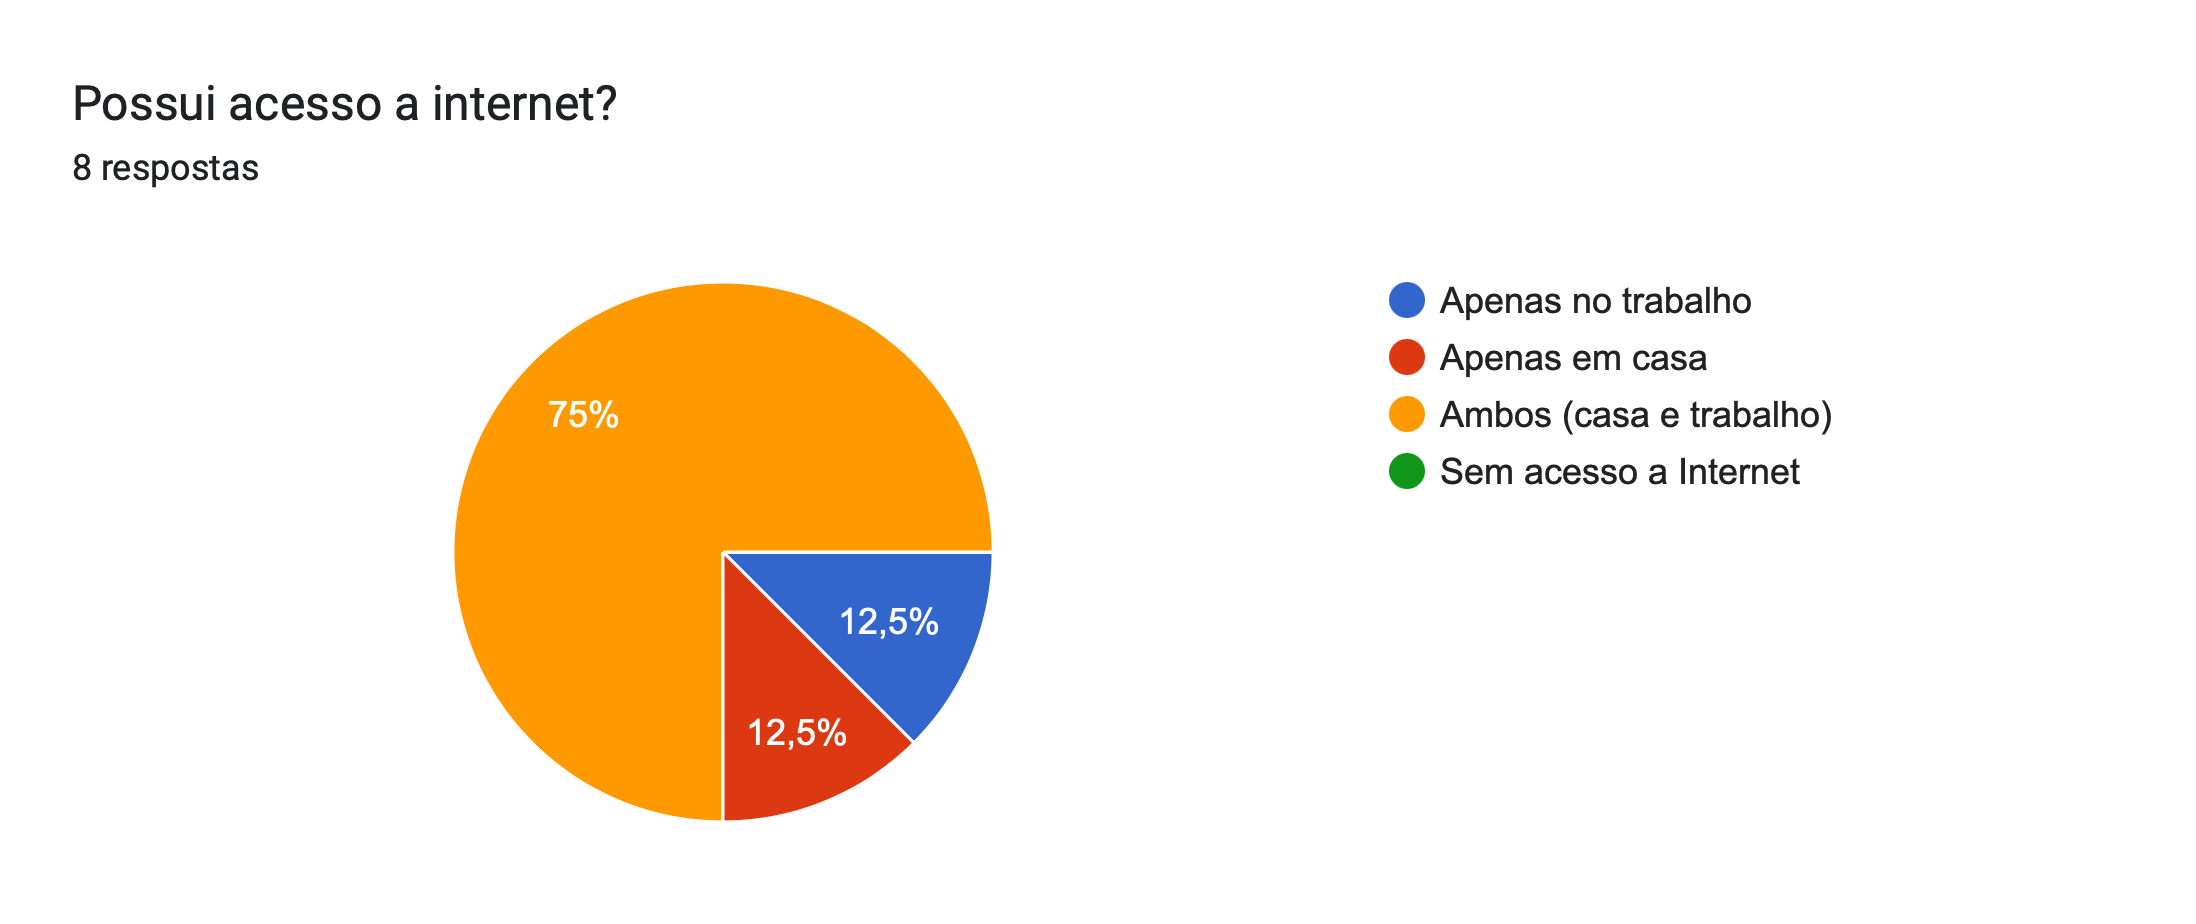
\includegraphics[scale=0.2]{figuras/resultados/acesso_internet.png}
    \label{fig:acesso_internet}
    \legend{Fonte: Eonay e Klenilmar (2024).}
\end{figure}

Para o uso da internet na prática docente podemos constatar que o acesso é de alcance a todos participantes seja ele no trabalho (12,5\%), em casa (12,5\%) ou ambos (75,0\%) os locais. Também foi levantado os dados do tipo de dispositivos que mais se utiliza para acesso a internet, onde representou 75,0\% o computador portátil. Também se tratando de portabilidade os \textit{smartphones} e \textit{tablets} também citados cada um com 12,5\% como dispositivos preferidos para esse uso, segue Figura \ref{fig:dispositivo_acesso_internet} com os referidos resultados.

\begin{figure}[h!]
    \caption{Dispositivo de acesso a Internet}
    \centering
    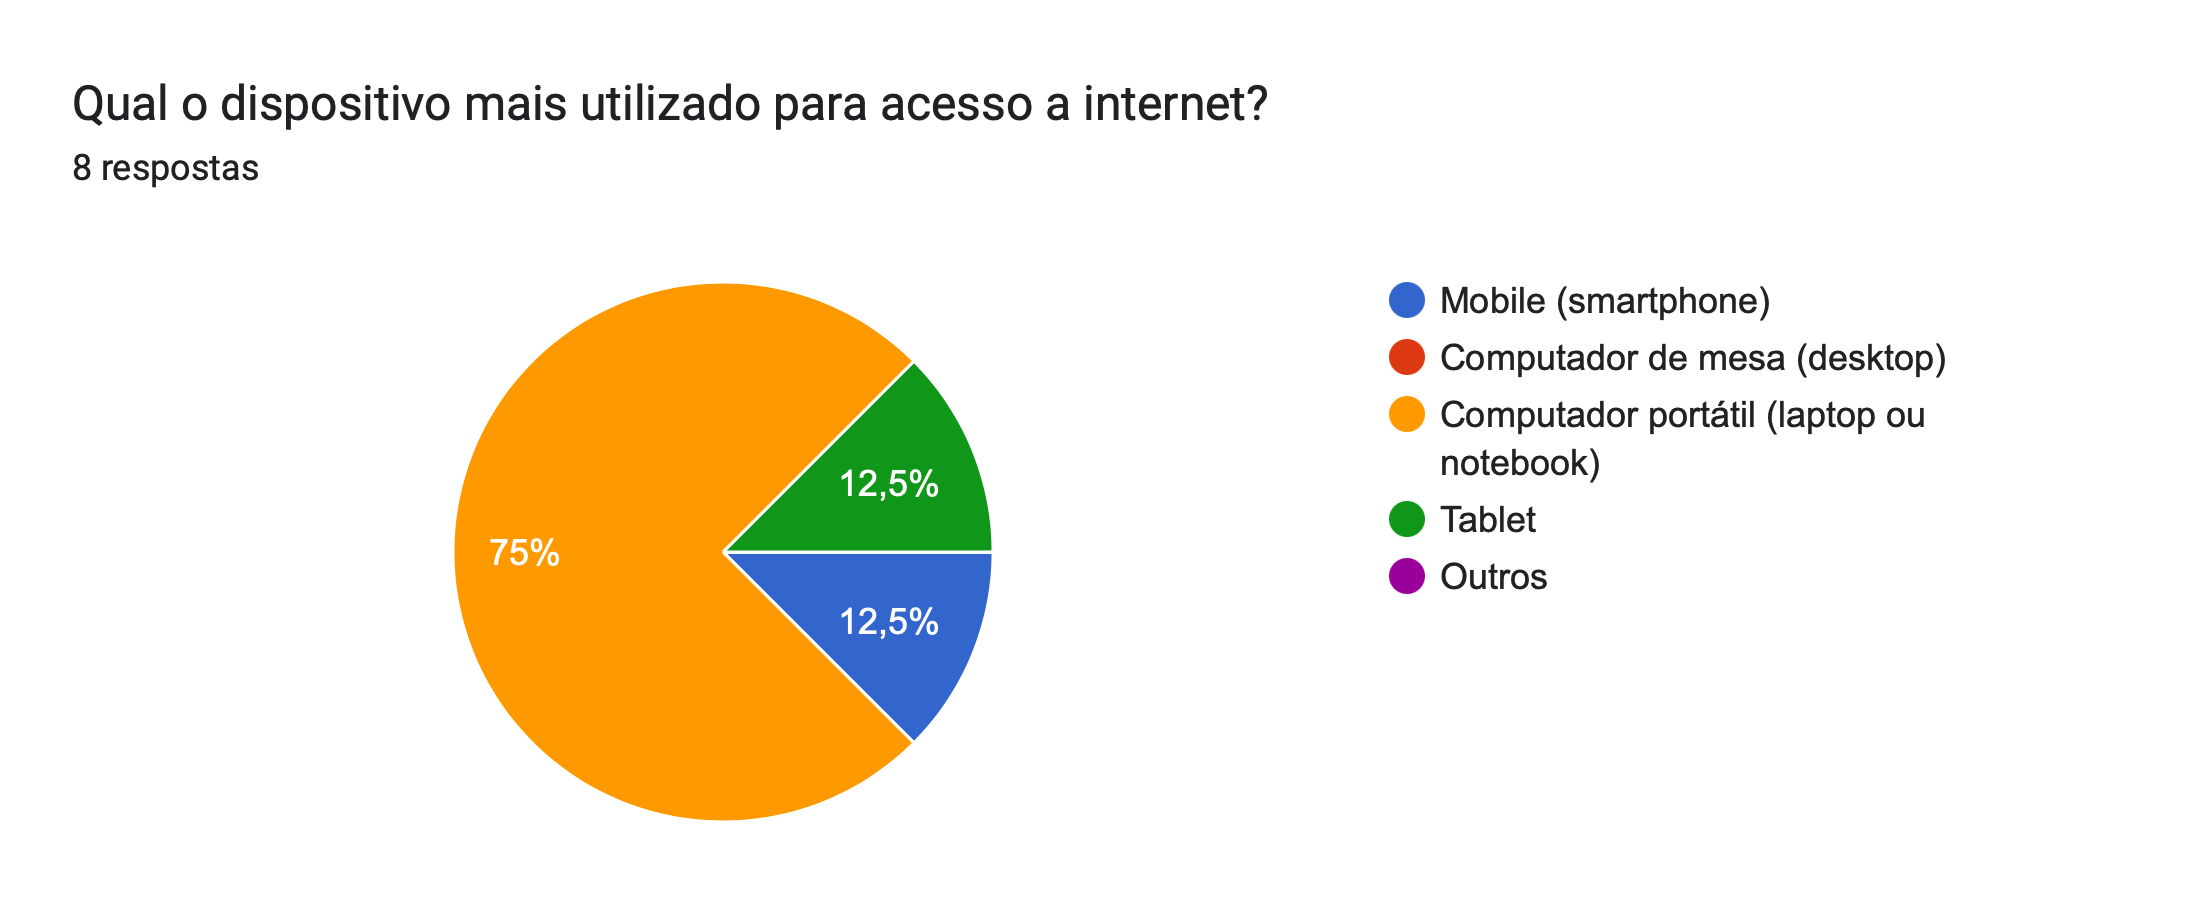
\includegraphics[scale=0.2]{figuras/resultados/dispositivo_acesso_internet.png}
    \label{fig:dispositivo_acesso_internet}
    \legend{Fonte: Eonay e Klenilmar (2024).}
\end{figure}



Considerando o uso das redes mundiais de computadores ou mais conhecida como a Internet, os principais dispositivos utilizados são os  móveis conforme indicativos supracitados é natural a utilização de softwares ou aplicativos para auxiliar a prática docente. O indicativo levantado direcionado a medir a frequência que se aplica tecnologias nos ambientes de ensino representado na Figura \ref{fig:softs_docencia}.

\begin{figure}[h!]
    \caption{Utilização de Softwares ou Aplicativos na Prática Docente}
    \centering
    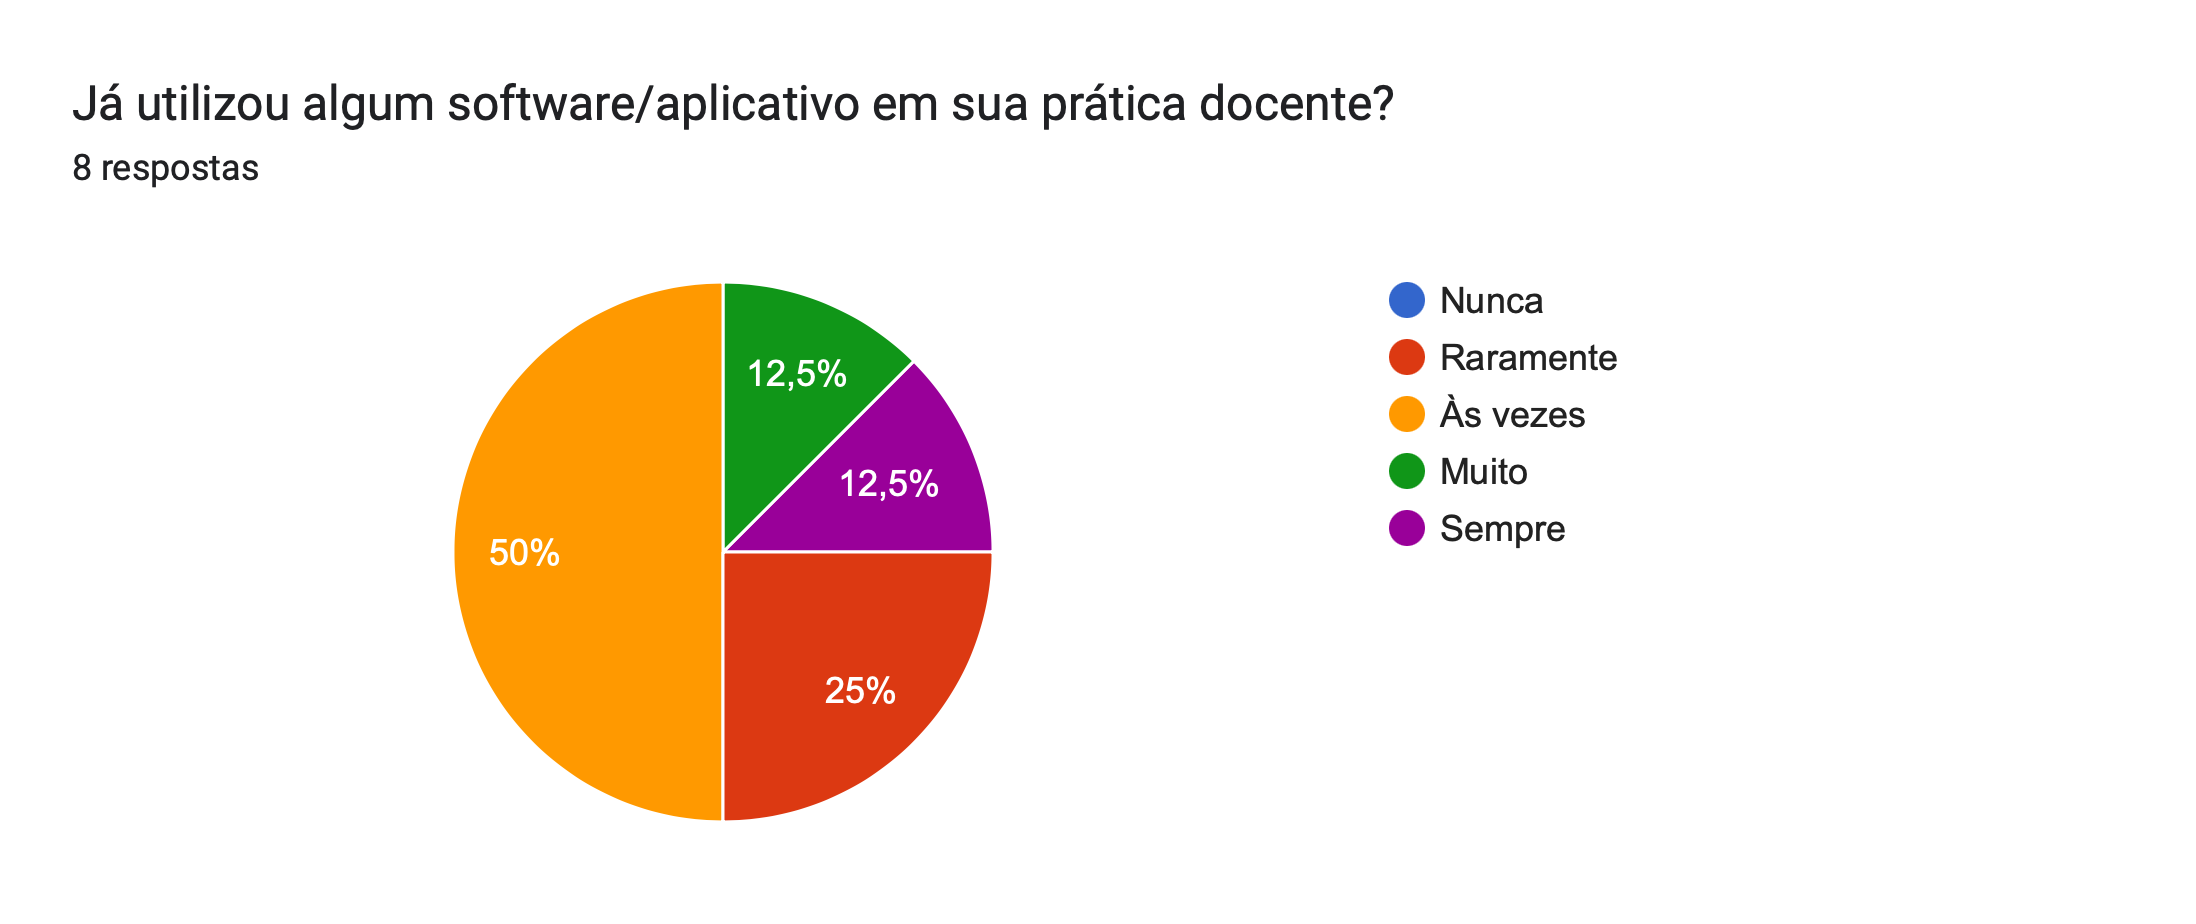
\includegraphics[scale=0.2]{figuras/resultados/software_pratica_docente.png}
    \label{fig:softs_docencia}
    \legend{Fonte: Eonay e Klenilmar (2024).}
\end{figure}



A análise do uso de ferramentas na prática docente revelou que 25,0\% dos participantes relataram utilizá-las raramente, enquanto 12,5\% afirmaram usá-las com frequência (muito) ou de forma constante (sempre) em suas aulas. A maioria, equivalente a 50,0\%, indicou utilizá-las apenas ocasionalmente (às vezes). Esses dados sugerem um indicativo de baixo uso de ferramentas tecnológicas nessa abordagem inicial e direcionada.

Quando questionados diretamente sobre a possibilidade de ensinar o conteúdo básico de matrizes utilizando alguma ferramenta tecnológica, 75,0\% dos educadores demonstraram concordância, enquanto 25,0\% preferiram se abster de responder, conforme ilustrado na Figura \ref{fig:ensino_matriz_app}. Esses resultados apontam para um potencial ainda pouco explorado no uso de ferramentas para o ensino desse conteúdo.

\begin{figure}[h!]
    \caption{Ensinar matriz utilizando software}
    \centering
    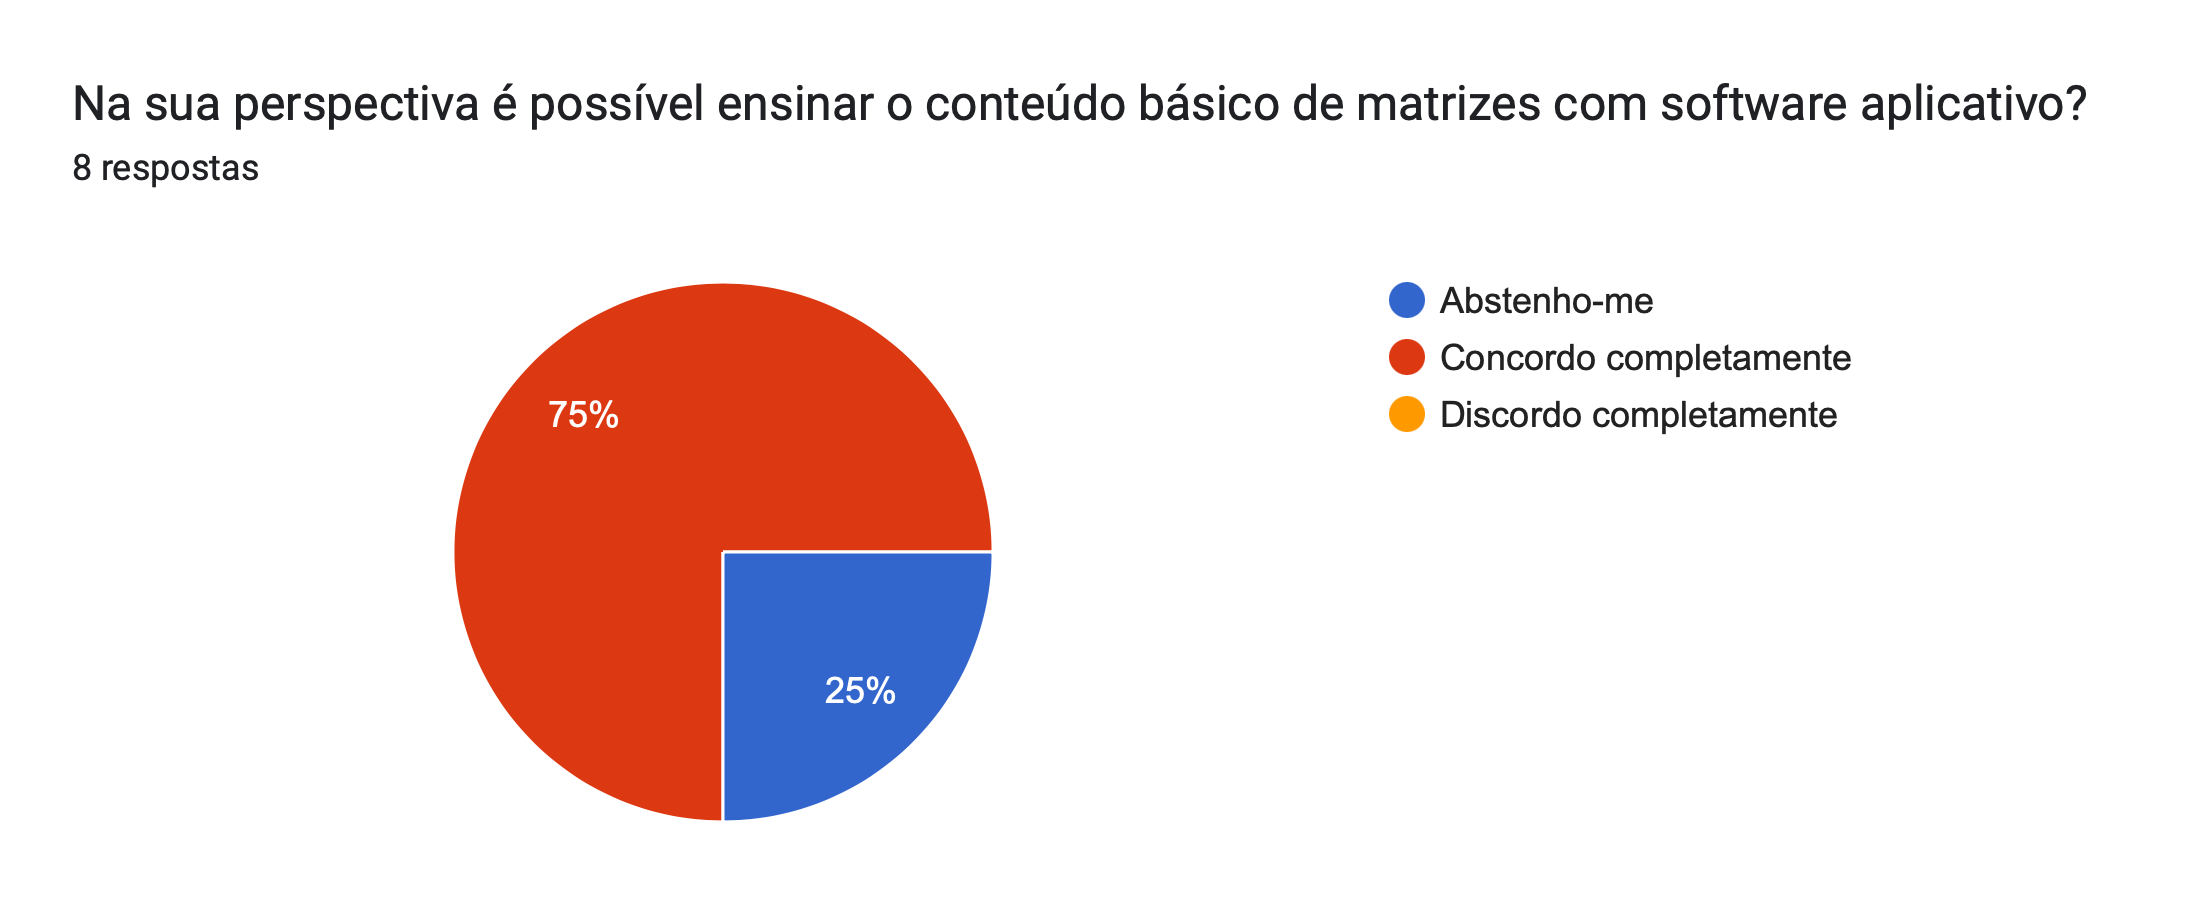
\includegraphics[scale=0.2]{figuras/resultados/ensino_matriz_app.png}
    \label{fig:ensino_matriz_app}
    \legend{Fonte: Eonay e Klenilmar (2024).}
\end{figure}


%De forma geral foi analisado a perspectiva dos docentes para uso de ferramentas diversas para o ensino não somente na matemática ou na área de exatas mas em um contexto maior, onde 12,5\% apontaram como regular ou muito satisfatório e 75,0\% como satisfatório.


De modo geral, foi analisada a perspectiva dos docentes quanto ao uso de ferramentas diversas no ensino não se limitando apenas à matemática ou às áreas de exatas, mas abrangendo um contexto mais amplo quantificado na Figura \ref{fig:soft_app_ensino}. Os resultados indicaram que 12,5\% dos participantes consideraram o uso dessas ferramentas como regular ou muito satisfatório, enquanto 75,0\% avaliaram como satisfatório. Esses dados refletem uma aceitação positiva, embora com margem para aprimoramento na integração dessas ferramentas no processo de ensino-aprendizagem.

\begin{figure}[h!]
    \caption{Uso geral de softwares/aplicativos no ensino}
    \centering
    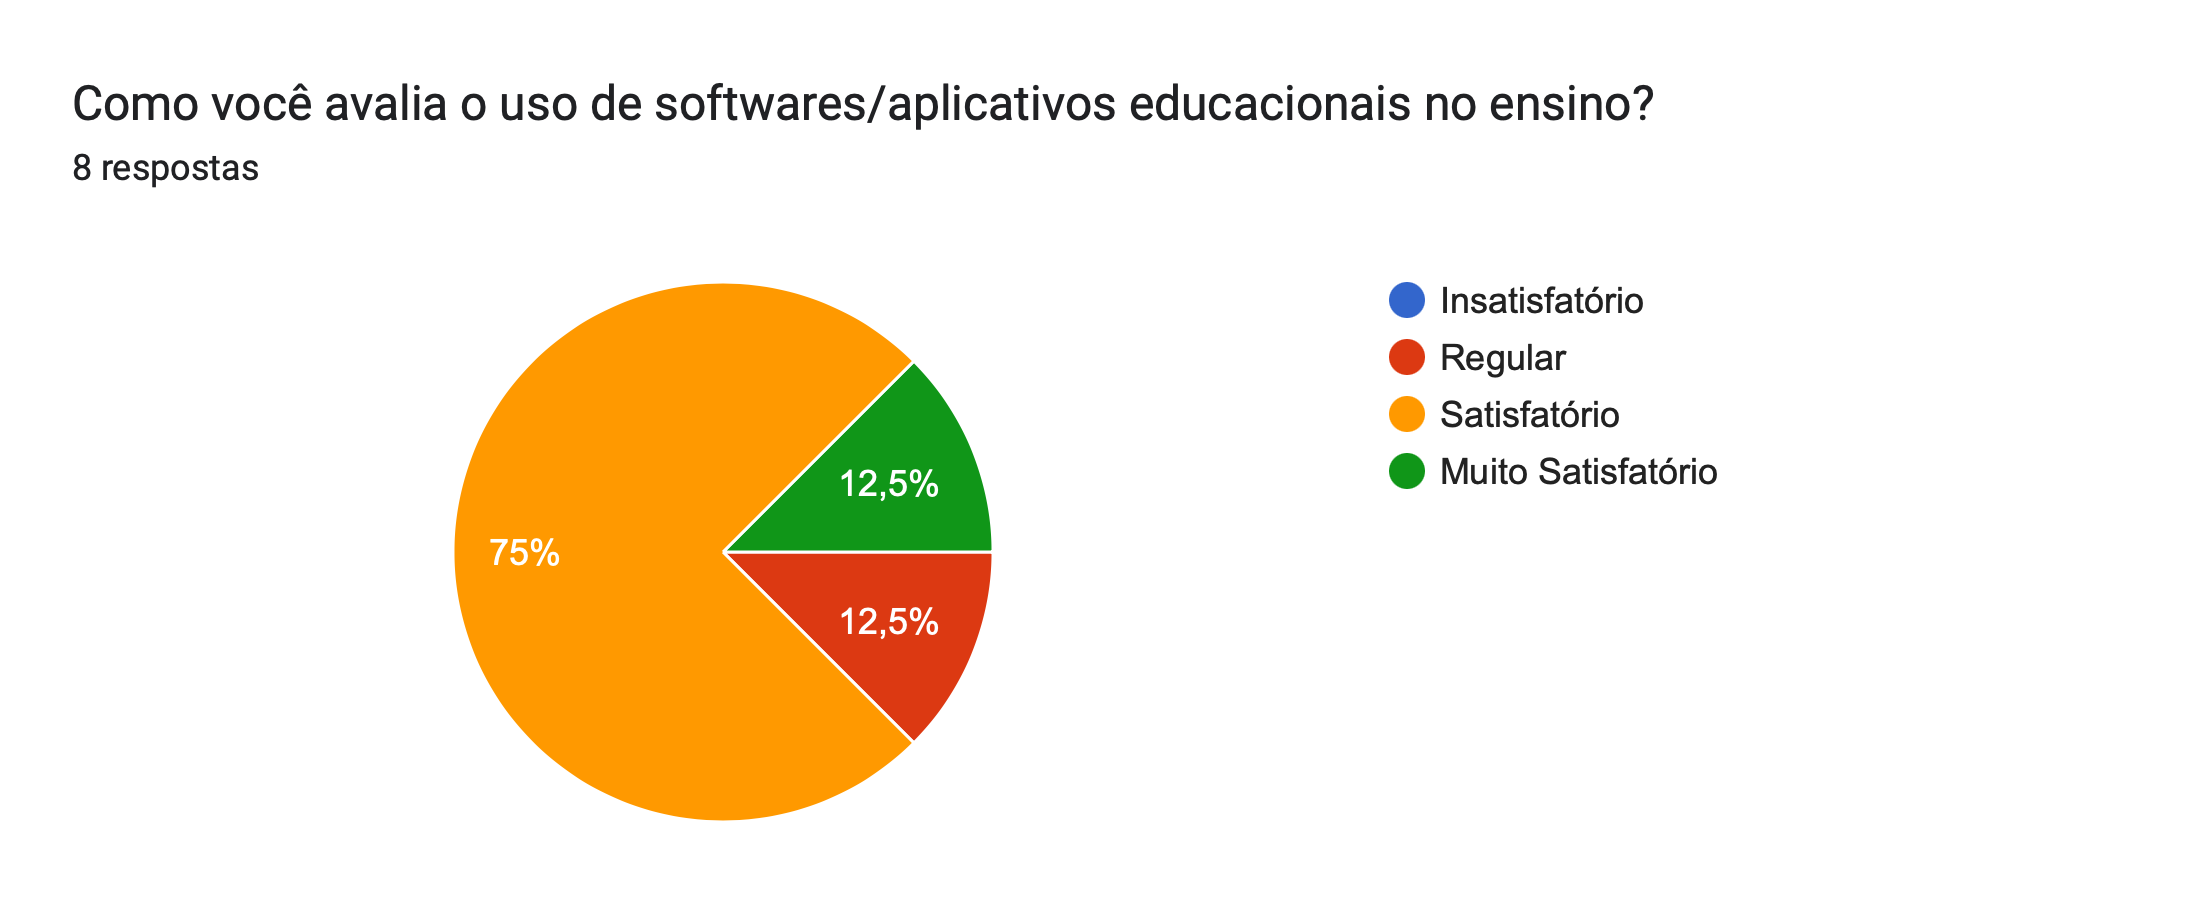
\includegraphics[scale=0.2]{figuras/resultados/app_ensino.png}
    \label{fig:soft_app_ensino}
    \legend{Fonte: Eonay e Klenilmar (2024).}
\end{figure}








\section{Produto Educacional}
\label{produto_educacional}

Disponibilização do produto educacional, software em formato REA (Recurso Educacional Aberto), tem objetivo de consolidação e aprimoramento pela comunidade acadêmica. O software foi desenvolvido no formato PWA é um acrônimo para \textit{Progressive Web Apps}, ou Aplicações Web Progressivas. A palavra \textit{progessiva} vem da ideia de \textit{Progressive Enhancement}, ou melhoria progressiva. Neste contexto, a ideia por trás da palavra \textit{progressiva} é condicionar uma aplicação a atender o maior número de pessoas possível, sob todos os aspectos \cite{pontes2018progressive}.


O formato PWA permite ampla compatibilidade com múltiplas plataformas, como Web, Android e iOS, e garante o funcionamento em diversos dispositivos, incluindo portáteis, como \textbf{tablets, smartphones e laptops}. Essa característica amplia o alcance e a acessibilidade da solução proposta.

O artefato, concebido como um Produto Educacional\footnote{http://eonay.ddns.net:8000}, publicado em repositório público, permitindo que outros docentes o utilizem em suas práticas pedagógicas. Dessa forma, ele pode ser aplicado em conjunto com diversas técnicas de ensino, tanto no ambiente educacional formal quanto no não formal, contribuindo para o desenvolvimento da aprendizagem dos educandos.

O Mathix é voltado para o currículo que aborda a componente de introdução a matrizes, utilizando uma aplicação em plataforma Web. A ferramenta promove uma abstração dos conceitos fundamentais de matrizes, estabelecendo uma relação prática entre teoria e aplicação. Ela é adaptável tanto para cursos presenciais quanto a distância, aproveitando a conectividade da rede mundial de computadores. É importante destacar que as características do produto foram definidas com base em um levantamento documental realizado durante a pesquisa, visando atender às demandas práticas da docência no processo de mediação do ensino-aprendizagem.

Com foco em auxiliar a prática docente, o produto educacional se distingui pela flexibilidade do software, podendo ser utilizado em ambientes formais e não formais de ensino. Além disso, ao seguir as orientações docentes de sustentação teórica, ele também pode ser empregado para estudos individuais. A ferramenta favorece ainda a integração com outras áreas de conhecimento, como estruturas de dados, programação, e mapeamento, sendo uma base útil para diversas aplicações e tarefas correlatas.


O produto também planeja-se a adaptação para uso do método de sala de aula invertida como objetivo contribuir e diversificar a adoção de tecnologias que podem agregar outros instrumentos para corroborar ou melhorar processo de ensino e aproximando mais o aluno do conteúdo. Para concepção do produto na perspectiva de \citeonline{kaplun2003material}, identificam-se três eixos correlacionados que se integram para o desenvolvimento de um Produto Educacional, segue: o eixo \textbf{conceitual}, o \textbf{pedagógico} e o \textbf{comunicacional}.


As três etapas paralelamente implementadas em quaisquer ferramenta proporcionam engajamento dos estudantes para alcançar o seu objetivo, neste sentido para \citeonline{kaplun2003material}, reforça o tripe conceitual, pedagógico e comunicacional para com  foco na metodologia aplicada no desenvolvimento na experiencia do usuário e na interface com usuário, deve-se também trabalhar em conjunto com outras práticas que remetam a um aprendizado significativo mediado por tecnologias.



A combinação dos eixos conceitual, pedagógico e comunicacional é essencial para criar uma \textbf{experiência de aprendizagem} eficaz e envolvente guiada pelo docente. O eixo conceitual estabelece os fundamentos teóricos, o pedagógico propõe as abordagens e estratégias de ensino, e o comunicacional garante que a interação entre o aluno e o conteúdo seja clara e envolvente.

Esses eixos interagem para fornecer uma abordagem holística, onde o aluno não só tem acesso ao conteúdo, mas é incentivado a se engajar ativamente com ele. No contexto da sala de aula invertida, isso se traduz em uma experiência onde o aluno assume maior responsabilidade por seu próprio aprendizado, com o apoio de ferramentas tecnológicas que potencializam o processo. A experiência do usuário e a interface com o aluno devem ser desenhadas de forma a facilitar esse engajamento, garantindo que a tecnologia seja um meio para um aprendizado significativo e não um fim em si mesma. Portanto, a colaboração entre esses três eixos é fundamental para o sucesso do produto educacional e para o desenvolvimento de uma aprendizagem mais rica e dinâmica.






Para desenvolvimento da proposta do produto alguns instrumentos foram utilizados, a princípio todas as ferramentas baseadas em \textbf{software livre}, segue: linguagem de programação Python, biblioteca Numpy para manipulação de vetores, framework para aplicações web Django e dentre outras para aplicações das regras de negócio conceituais aplicadas de forma pedagógica com uma interface acessível, segue a interface principal na Figura \ref{fig:home_mathix}:

\begin{figure}[h!]
    \caption{Interface principal Mathix}
    \centering
    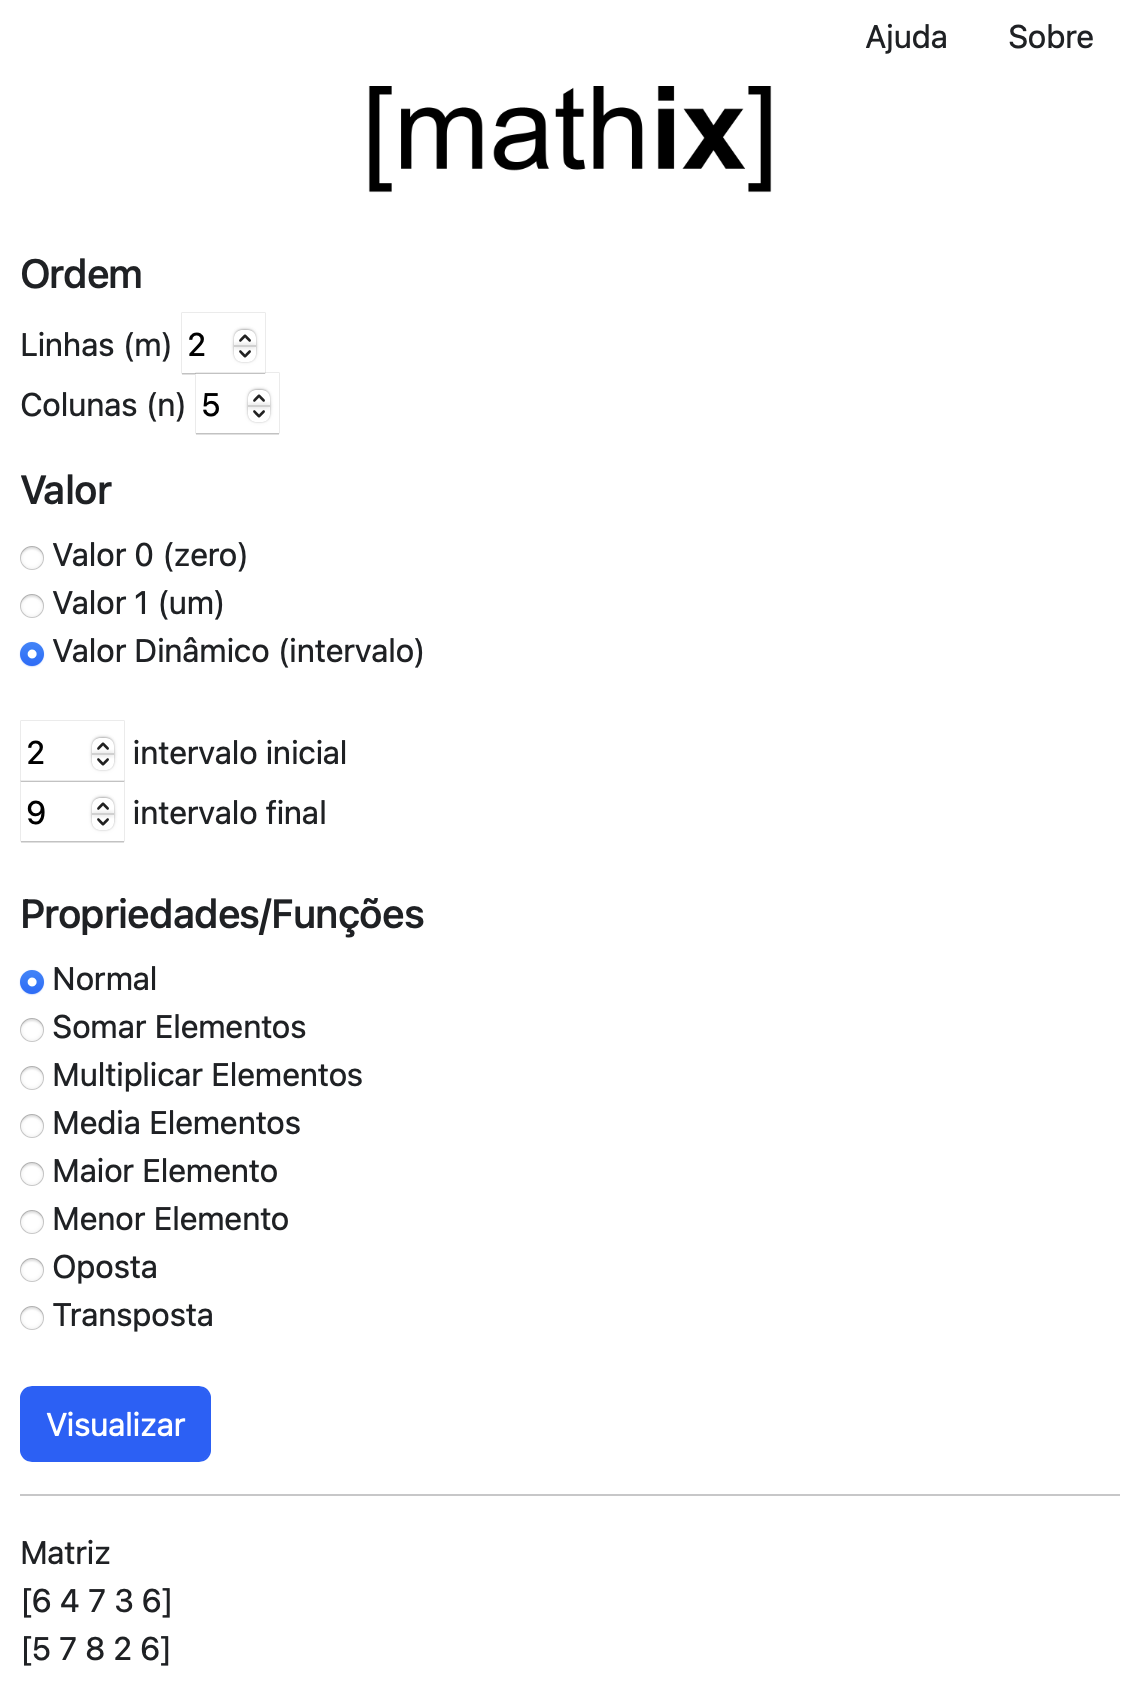
\includegraphics[scale=0.4]{figuras/mathix-home.png}
    \label{fig:home_mathix}
    \legend{Fonte: Eonay e Klenilmar (2024).}
\end{figure}

Se propôs o nome para a ferramenta de \textbf{Mathix} em referencia a palavra matriz e matemática com um arranjo em conjunto a outra referência ao número 9 (nove) representado algarismo romano, segue na Figura \ref{fig:logo_mathix} a proposição de logo.

\begin{figure}[h!]
    \caption{Logomarca Mathix}
    \centering
    
\includegraphics[scale=0.4]{figuras/mathix_logo.png}
    \label{fig:logo_mathix}
    \legend{Fonte: Eonay e Klenilmar (2024).}
\end{figure}

Outro ponto a ressaltar é que este trabalho contou com a colaboração do \textbf{GPTICAM} (Grupo de Pesquisa em Tecnologias da Informação e Comunicação na Amazônia) onde dentre as linhas de pesquisa a Engenharia de Software corroborar com o desenvolvimento do produto educacional. Ressaltar que durante o andamento dos trabalhos outras atividades ou produtos podem ser derivados da pesquisa assim como a inclusão de novos recursos ao Mathix.


O objeto educacional final será um Recurso Educacional Aberto (REA) que assegura a utilização, modificação e reutilização do produto para futuras pesquisas na área da educação e consequentemente sua evolução, melhorias e agregação para novas versões ou aplicação em conjunto com novos projetos. O conceito de REA segundo \cite{nobre2016incorporar}:


\begin{citacao}
Os materiais de ensino, aprendizagem e investigação em quaisquer suportes, digitais ou outros, que se situem no domínio público ou que tenham sido divulgados sob licença aberta que permite acesso, uso, adaptação e redistribuição gratuitos por terceiros, mediante nenhuma restrição ou poucas restrições. O licenciamento aberto é construído no âmbito da estrutura existente dos direitos de propriedade intelectual, tais como se encontram definidos por convenções internacionais pertinentes, e respeita a autoria da obra \cite{nobre2016incorporar}.
\end{citacao}

Contudo o resultado visa contribuir para prática docente tornando-a mais atrativa aos educandos, podendo ser empregado em múltiplas áreas que se utilizam do conceito de matrizes, pelas características pode ser agregada em outras plataformas como AVA (Ambiente Virtual de Aprendizagem) entre outras para fortalecimento do ensino.




\section{Avaliação do Produto Educacional}
\label{avaliacao_pe}

Após a disponibilização do produto educacional Mathix para uso e testes, recebemos diversos \textit{feedbacks} de profissionais da área educacional, os quais avaliaram a ferramenta e a sua aplicabilidade no ensino, considerando seu modelo de Produto Mínimo Viável (PMV). A seguir, apresentamos os resultados obtidos a partir da aplicação de um questionário sobre o uso da ferramenta no ensino, conforme mostrado na Tabela \ref{tab:p1}.


%%% Pergunta 01

\begin{table}[h!]
    \centering
    \caption{O produto educacional deve ser utilizado no ensino}
    \begin{tabular}{c|c|c}
        \textbf{Resposta} &	\textbf{Absoluto} & \textbf{Relativo} \\
        \hline
        Sim & 7 & 87,5\% \\
        \hline
        Não & 1 & 12,5\% \\
    \end{tabular}
    \legend{Fonte: Eonay e Klenilmar (2024).}
    \label{tab:p1}
\end{table}


De acordo com os dados da Tabela \ref{tab:p1}, aproximadamente 87,5\% dos participantes acreditam que a ferramenta deve ser utilizada no ensino, enquanto 12,5\% são contrários ao seu uso no contexto educacional. Além disso, a questão sobre a aderência do produto à prática docente também foi analisada. Considerando aspectos como confiabilidade e facilidade de uso, já que se tratava do primeiro contato dos participantes com a ferramenta, os resultados indicaram que 87,5\% utilizariam a ferramenta em suas aulas, enquanto 12,5\% não optariam por usá-la, como representado na Figura \ref{fig:p2}


%%% Pergunta 02
\begin{figure}[h!]
    \caption{Utilizaria o PE em sua prática docente}
    \centering
    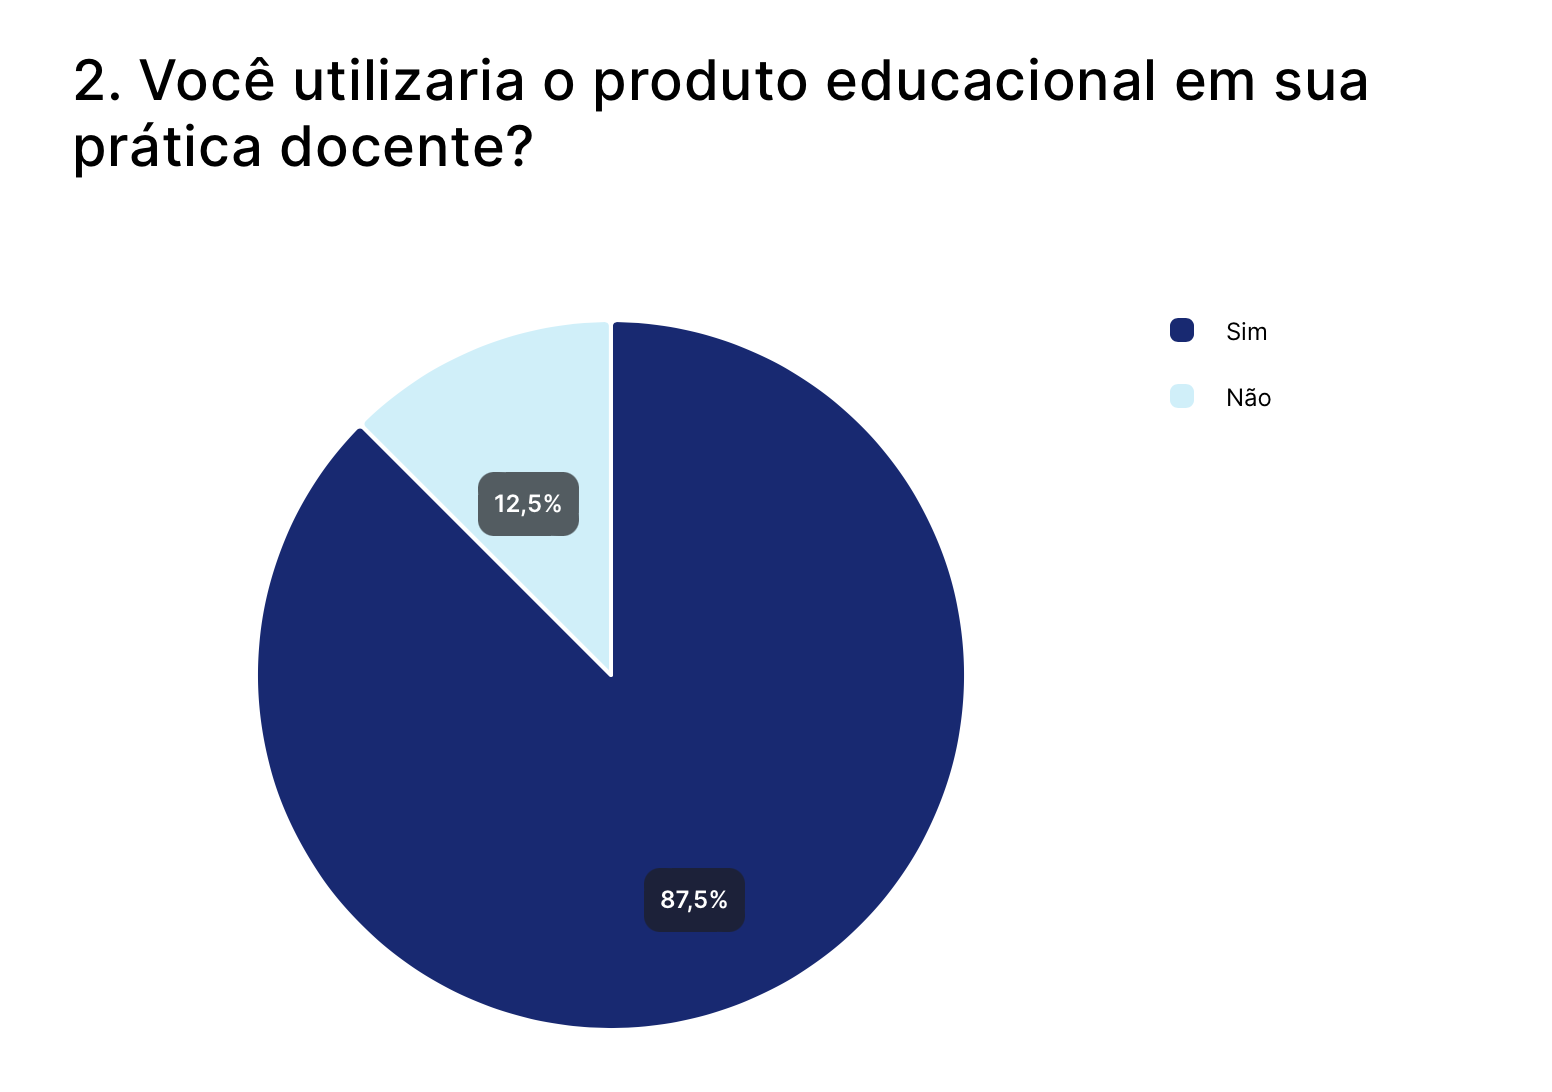
\includegraphics[scale=0.3]{figuras/resultados/p2.png}
    \label{fig:p2}
    \legend{Fonte: Eonay e Klenilmar (2024).}
\end{figure}




%%% Pergunta 03
Outro ponto relevante foi a avaliação da satisfação dos participantes em relação ao uso do produto educacional, que foi disponibilizado na forma de software/aplicativo. Vale destacar que todos os participantes utilizaram a plataforma de maneira independente, sem restrições e, em alguns casos, de forma concorrente com outras ferramentas. Os resultados, apresentados na Tabela \ref{tab:p3}, mostram que 62,5\% consideraram o produto Satisfatório, 25,0\% o avaliaram como Muito Satisfatório e 12,5\% o classificaram como Regular em relação à satisfação com o uso da ferramenta.


\begin{table}[h!]
    \centering
    \caption{Surgiu alguma dificuldade em manusear o produto educacional}
    \begin{tabular}{c|c|c}
        \textbf{Resposta} &	\textbf{Absoluto} & \textbf{Relativo} \\
        \hline
        Sim & 6 & 75,0\% \\
        \hline
        Não & 2 & 25,0\% \\
    \end{tabular}
    \legend{Fonte: Eonay e Klenilmar (2024).}
    \label{tab:p3}
\end{table}



%%% Pergunta 04

A seguir, foi investigada a dificuldade de manuseio da plataforma, levando em conta seu formato livre, interface clean (limpa) e a ausência de manuais de instrução. A Tabela \ref{tab:p3} resume os indicadores de dificuldade relacionados a essa questão. Vale ressaltar que uma características de plataforma é a questão da usabilidade, configurabilidade, extensibilidade e instalabilidade.


A satisfação de utilizar o software representado na Tabela \ref{tab:p4}, em utiliza-ló sem a necessidade de manuais está diretamente ligada à sua interface intuitiva e à experiência fluida que oferece. Quando se trata de um Produto Mínimo Viável (PMV), a simplicidade e funcionalidade se destacam, tornando o uso natural e acessível, mesmo sem um guia extenso. Para plataformas educacionais que abstraem teorias complexas, o software se torna uma ferramenta poderosa ao transformar conceitos abstratos em experiências práticas e compreensíveis. Isso permite que os usuários, sejam alunos ou educadores, interajam de forma eficaz com o conteúdo, sem sobrecarga cognitiva, promovendo um aprendizado mais envolvente e eficiente.


\begin{table}[h!]
    \centering
    \caption{De forma geral, sua satisfação ao utilizar o produto educacional na forma software/aplicativo}
    \begin{tabular}{c|c|c}
        \textbf{Resposta} &	\textbf{Absoluto} & \textbf{Relativo} \\
        \hline
        Satisfatório & 5 & 62,5\% \\
        \hline
        Muito Satisfatório & 2 & 25,0\% \\
        \hline
        Regular & 1 & 12,25\% \\
        \hline
        Insatisfatório & 0 & 0,0\% \\
    \end{tabular}
    \legend{Fonte: Eonay e Klenilmar (2024).}
    \label{tab:p4}
\end{table}


%%% Pergunta 05

O produto educacional Mathix tem como objetivo auxiliar a prática docente, especialmente no ensino de matrizes, oferecendo uma plataforma rápida e flexível. Perguntou-se aos participantes se o produto correspondeu às expectativas relacionadas ao seu propósito, e os resultados estão apresentados na Tabela \ref{tab:p5}. Dentre os participantes, 62,5\% consideraram o produto Satisfatório em termos de seu propósito, 12,5\% o avaliaram como Muito Satisfatório, enquanto 12,5\% classificaram-no como Regular, evidenciando que a ferramenta ainda se encontra em sua fase inicial e possui funcionalidades limitadas.


\begin{table}[h!]
    \centering
    \caption{A aplicação propôs a fazer a função para qual foi desenvolvido}
    \begin{tabular}{c|c|c}
        \textbf{Resposta} &	\textbf{Absoluto} & \textbf{Relativo} \\
        \hline
        Satisfatório & 6 & 62,5\% \\
        \hline
        Muito Satisfatório & 1 & 12,5\% \\
        \hline
        Regular & 1 & 12,25\% \\
        \hline
        Insatisfatório & 0 & 0,0\% \\
    \end{tabular}
    \legend{Fonte: Eonay e Klenilmar (2024).}
    \label{tab:p5}
\end{table}



%%% Pergunta 06

Por fim, de forma opcional, foi solicitado aos participantes que dessem sugestões de melhorias para o produto educacional, com base em suas experiências. Quatro relatos construtivos foram obtidos, abordando aspectos relacionados à Experiência do Usuário (UX) e à Interface do Usuário (UI), os quais foram considerados importantes para aprimorar a usabilidade e a efetividade do produto.


\begin{citacao}

    \item "Parabéns pela iniciativa, inserir outras tarefas que se utiliza matrizes";

    \item "Os resultados poderiam ficar ao lado em vez de baixo por conta do local de exibição na tela";

    \item "Inicialmente não deve-se utilizar para não produzir efeito de facilidade, mas pode ser utilizado para atividades";

    \item "Em uma perspectiva geral eu achei que o Mathix tem uma estética simples e clara, e fácil de usar. Mas pensando em um usuário em nível inicial, deixar visíveis os rótulos dos campos na tela facilitariam o uso (os mesmos do menu Ajuda). Nos resultados disponibilizar uma curta explicação das Propriedades. E caso o usuário deixe os campos linhas e colunas vazios, informar que os campos precisam ser preenchidos";

\end{citacao}







\subsection{Avaliação de Interface de Usuário (UI)}
\label{avaliacao_ui}

Em conjunto a avaliação do PE foi analisado a interface para com características que variam em percentuais fixos que varias a cada 20\% para cada opção de resposta, inicialmente foi questionado a possibilidade de recomendação a seus pares (outros docentes), Tabela \ref{tab:ui-1} segue: 

\begin{table}[h!]
    \centering
    \caption{Qual é a probabilidade de você recomendar o Mathix para outros docentes}
    \begin{tabular}{c|c|c}
        \textbf{Resposta} &	\textbf{Absoluto} & \textbf{Relativo} \\
        \hline
        Muito alto 75\% & 5 & 62,5\% \\
        \hline
        Extremamente alto 100\% & 2 & 25,0\% \\
        \hline
        Talvez sim, talvez não 50\% & 1 & 12,5\% \\
        \hline
        Baixo 25\% & 0 & 0,0\% \\
        \hline
        Nenhuma 0\% & 0 & 0,0\% \\
    \end{tabular}
    \legend{Fonte: Eonay e Klenilmar (2024).}
    \label{tab:ui-1}
\end{table}

Obtivemos cerca de 62,5\% dos participantes que recomendariam a outros colegas docentes com intensidade de muito alta e 25\% optaram por recomendar de forma extremamente alta, seguido de 12,5\% que têm duvidas sobre a recomendação. Consequentemente recomenda-se algo que desperte interesse e que seja performático na perspectiva do usuário, na Tabela \ref{tab:ui-2} foi analisado a questão do desempenho.


\begin{table}[h!]
    \centering
    \caption{Qual é a sua opinião geral sobre o desempenho do Mathix}
    \begin{tabular}{c|c|c}
        \textbf{Resposta} &	\textbf{Absoluto} & \textbf{Relativo} \\
        \hline
        Bom & 4 & 50,0\% \\
        \hline
        Ótimo & 3 & 37,5\% \\
        \hline
        Regular & 1 & 12,5\% \\
        \hline
        Ruim & 0 & 0,0\% \\
        \hline
        Péssimo & 0 & 0,0\% \\
    \end{tabular}
    \legend{Fonte: Eonay e Klenilmar (2024).}
    \label{tab:ui-2}
\end{table}

No contexto do desempenho em plataformas web, é essencial destacar a relevância desse aspecto para a experiência do usuário. A velocidade e a eficiência de um site ou aplicação têm impacto direto na usabilidade e na satisfação dos usuários. Estudos indicam que a otimização do desempenho não apenas melhora a experiência do usuário, mas também influencia fatores cruciais como taxas de conversão, retenção e satisfação geral.

De acordo com uma pesquisa da Google, um atraso de apenas um segundo no tempo de carregamento de uma página pode reduzir as conversões em até 20\% \cite{google2018speed}. Esses dados reforçam a importância de priorizar melhorias de performance como parte das estratégias de desenvolvimento e manutenção de plataformas digitais. Outro aspecto analisado é com relação a travamentos e falhas mostrado na Tabela \ref{tab:ui-3}:



\begin{table}[h!]
    \centering
    \caption{Com que frequência o Mathix costuma congelar ou falhar}
    \begin{tabular}{c|c|c}
        \textbf{Resposta} &	\textbf{Absoluto} & \textbf{Relativo} \\
        \hline
        Ainda não sei & 5 & 62,5\% \\
        \hline
        Nunca & 2 & 25,0\% \\
        \hline
        Ocasionalmente & 1 & 12,5\% \\
        \hline
        Frequentemente & 0 & 0,0\% \\
        \hline
        Constantemente & 0 & 0,0\% \\
    \end{tabular}
    \legend{Fonte: Eonay e Klenilmar (2024).}
    \label{tab:ui-3}
\end{table}

O dados corroboram com a avaliação de desempenho e revelam que 62,5\% durante o uso optaram por "Ainda não sei", e 25,0\% como "Nunca" o que leva a concluir sobre a estabilidade do software, também responderam com 12,5\% como ocasionalmente obtiveram alguma instabilidade durante os testes.

Se tratando do uso, a investigação computou a informação sobre a facilidade baseada na interface e interatividade do participante Tabela \ref{tab:ui-4}, onde 50\% dos participantes afirmaram ser extremamente fácil e 37,5\% como muito fácil, afirmando simplicidade da ferramenta, ainda 12,5\% acreditam não ser muito fácil utilizar.


\begin{table}[h!]
    \centering
    \caption{Quão fácil de ser usada é a interface do Mathix}
    \begin{tabular}{c|c|c}
        \textbf{Resposta} &	\textbf{Absoluto} & \textbf{Relativo} \\
        \hline
        Extremamente fácil & 4 & 50,0\% \\
        \hline
        Muito fácil & 3 & 37,5\% \\
        \hline
        Não muito fácil & 1 & 12,5\% \\
        \hline
        Moderadamente fácil & 0 & 0,0\% \\
        \hline
        Nada fácil & 0 & 0,0\% \\
    \end{tabular}
    \legend{Fonte: Eonay e Klenilmar (2024).}
    \label{tab:ui-4}
\end{table}

Uma das dificuldade que os usuários enfrentam é com relação aos requisitos e instalação de ferramenta para utilização, assim a Tabela \ref{tab:ui-5} traz 87,5\% informando facilidade extrema e de formada moderada 12,5\% em instalar e configurar o PE para operação.

\begin{table}[h!]
    \centering
    \caption{Quão fácil foi instalar o nosso Mathix}
    \begin{tabular}{c|c|c}
        \textbf{Resposta} &	\textbf{Absoluto} & \textbf{Relativo} \\
        \hline
        Extremamente fácil & 7 & 87,5\% \\
        \hline
        Moderadamente fácil & 1 & 12,5\% \\
        \hline
        Nada fácil & 0 & 0,0\% \\
    \end{tabular}
    \legend{Fonte: Eonay e Klenilmar (2024).}
    \label{tab:ui-5}
\end{table}

De forma optativa foi perguntado quais aspectos do Mathix precisamos melhorar e de forma a correlacionar e categorizar os \textit{feedback} das respostas:

\begin{citacao}
    \item "Uma interface um pouco mais intuitiva no processo construtivo das matrizes, considerando os valores específicos dos termos e uma melhor visualização gráfica, porém é satisfatório considerando as propostas de operações". \textbf{Categoria}: Interface.
    
    \item "Tutorial sobre o uso do Mathix". \textbf{Categoria}: Manual.
    
    \item "Possibilidade de impressão de tarefas e inserir outras funções para com as matrizes". Categoria: Interface e Funcionalidade.
    
    \item "Gostaria que o Mathix além de mostrar o resultado final, mostrasse o passo a passo daquele resultado. Senti falta da matriz inversa" . \textbf{Categoria}: Interface e Funcionalidade.
    
    \item "Como o foco do Mathix é abordar matrizes em um nível introdutório, considero que para iniciantes alguns esclarecimentos poderiam ficar fixados na interface (para facilitar o uso). Por exemplo: Valor Dinâmico (intervalo): Especifique um valor (aceita valores positivos e negativos). Seria interessante exibir uma explicação curta no resultado, para ajudar o estudante no aprendizado. Por exemplo, Matriz oposta (Para os elementos correspondentes inverte-se o sinal do valor)". \textbf{Categoria}: Interface e Manual.
    
    \item "Adicionar outras operações com matrizes". \textbf{Categoria}: Funcionalidade.
\end{citacao}


Estas categorias percorridas trazem um indicador evolutivo do ponto de partida do produto educacional de \textbf{Interface, Manual e Funcionalidade} que podem e devem ser trabalhadas futuramente em outras versões. Por fim foi solicitado aos participantes um parecer final de avaliação da interface de forma optativa, segue:

\begin{citacao}

\item "Utilizaria como ferramenta complementar e não como ferramenta principal pois apenas mostra o resultado e falta de um viés didático. Por exemplo, muita vezes sem o auxilio do professor, o aluno o utilizaria para verificar algumas soluções. Mas o porque? Para que? ainda estão indefinidos. Gostei da iniciativa, mas o produto sem mostrar o passo a passo da solução e sem mostrar a matriz inversa, fica incompleto. Outra coisa, os elementos são apenas com valores inteiros";

\item "Simples, possibilita gerar item para exercícios";

\item "É um ferramenta que pode ser aplicadas para o aluno exercitar em casa e para uso no projetor para as aulas presenciais ou EAD";

\item "Considerando as propriedades propostas, seria altamente benéfico incluir a demonstração de outras operações e propriedades fundamentais que os alunos encontram ao ter o primeiro contato com o conteúdo de matrizes. Isso tornaria a experiência com o produto mais rica e envolvente, facilitando uma compreensão mais abrangente e prática do tema";

\item "Achei a ferramenta fácil de usar, tem uma estética simples e minimalista, incorpora um conjunto significativo de propriedades/funções de matrizes".

\end{citacao}

De forma geral a avaliação de 1 a 10 para a interface do produto educacional na Figura \ref{fig:ui-8}, representado na escala radial que demonstra um alto índice de satisfação no intervalo entre 6 e 9 como resultado indicador de aceitação pelos participantes.

\begin{figure}[h!]
    \caption{Grau de Satisfação do PE (UI)}
    \centering
    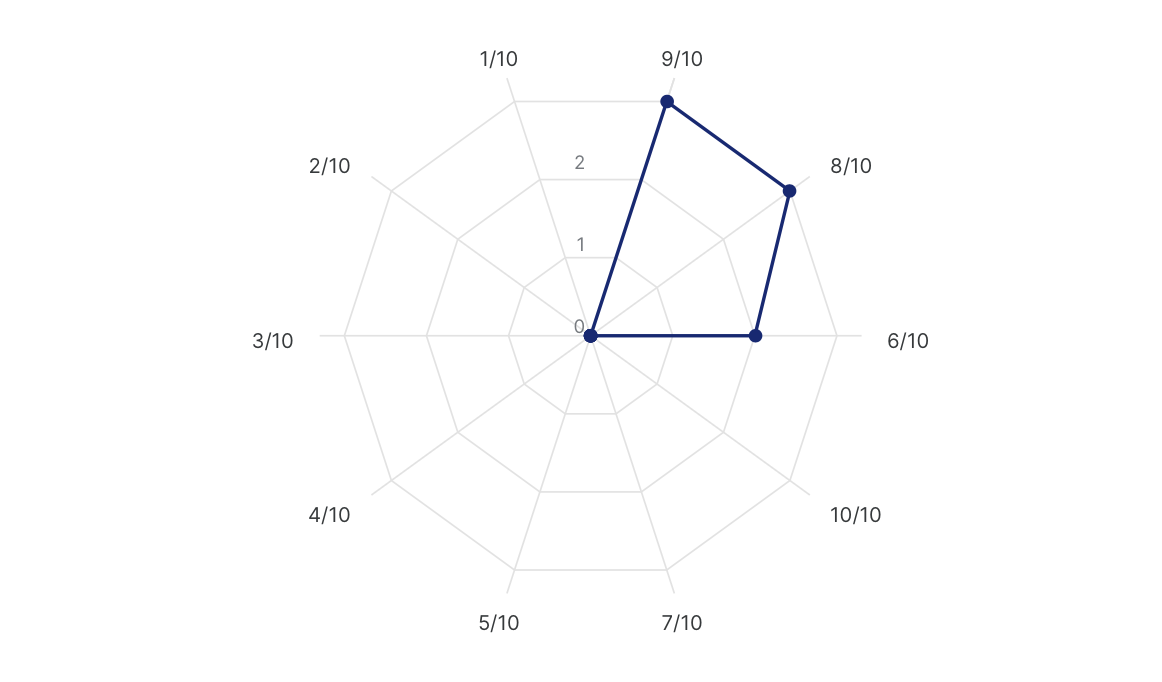
\includegraphics[scale=0.5]{figuras/resultados/satisfacao_ui.png}
    \label{fig:ui-8}
    \legend{Fonte: Eonay e Klenilmar (2024).}
\end{figure}











\subsection{Avaliação de Experiência de Usuário (UX)}
\label{avaliacao_ux}


Também em conjunto com a avaliação do PE foi analisado a experiencia do usuário para com características como \textbf{atratividade, controle, eficiência, estimulação, novidade e perspicuidade} para certos itens de cada respectivo grupo, cada opção de resposta variando entre -5 e 5 sendo, menor satisfação para maior satisfação respectivamente.

A Tabela \ref{fig:ux-1} retrata a avaliação de atratividade onde na visão dos participantes o produto educacional se mostrou agradável, atraente, atrativo e bom na avaliação media dos participantes. Para \citeonline{Tractinsky2000} "A atratividade de software está relacionada à combinação de estética, usabilidade e funcionalidade, sendo um fator crítico para a aceitação e retenção de usuários".

\begin{figure}[h!]
    \caption{Você gostou do produto}
    \centering
    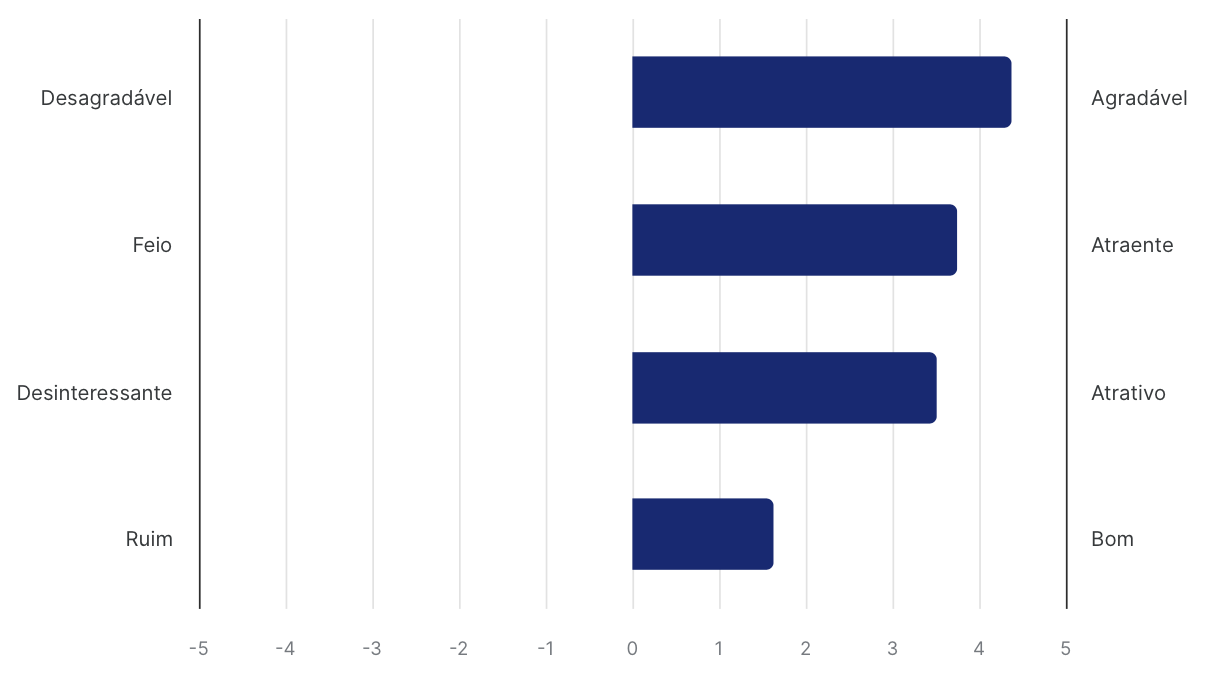
\includegraphics[scale=0.4]{figuras/resultados/ux-1.png}
    \label{fig:ux-1}
    \legend{Fonte: Eonay e Klenilmar (2024).}
\end{figure}

Alguns comentários deixados sobre atratividade apos a avaliação dos participantes:

\begin{citacao}
\item "Poderia ter um aplicativo específico";
\item "Funciona no celular e tablet de forma igual";
\item "Estudantes gostam quando professores saem do modelo convencional (aula explicativa e exercícios em papel). Então, a ferramenta é atrativa e interessante para estudantes aprender praticando".
\end{citacao}

Na Figura \ref{fig:ux-3} a avaliação de controle sobre o produto educacional eleva as características que atende a necessidade de forma segura.

\begin{figure}[h!]
    \caption{Você se sente no controle da situação durante a interação}
    \centering
    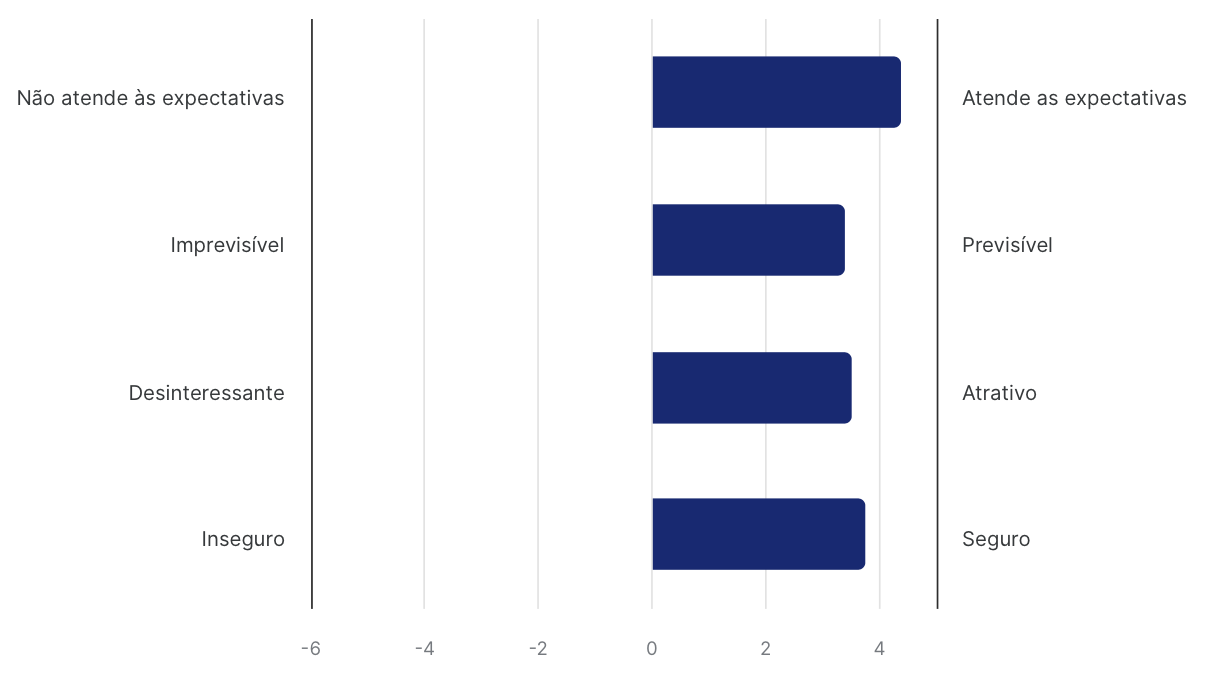
\includegraphics[scale=0.4]{figuras/resultados/ux-3.png}
    \label{fig:ux-3}
    \legend{Fonte: Eonay e Klenilmar (2024).}
\end{figure}

Um dos participantes deixou um comentário sobre o controle na avaliação:
"Lembrando que existem outras caracteristicas de matrizes que o sisteminha não contempla"\footnote{O texto encontra-se fidedigno ao texto coletado, caracteristicas entenda como características, sisteminha entenda como sistema ou produto educacional}. Reforço que o MPV é uma proposta inicial e deve ser continuado em trabalhos futuros pela comunidade. A avaliação do ponto de vista de eficiência também aponta na Figura \ref{fig:ux-5} indicativo de praticidade e rapidez que corrobora com a avaliação de desempenho da analise de interface.

\begin{figure}[h!]
    \caption{O produto pode ser utilizado de maneira fácil e eficiente}
    \centering
    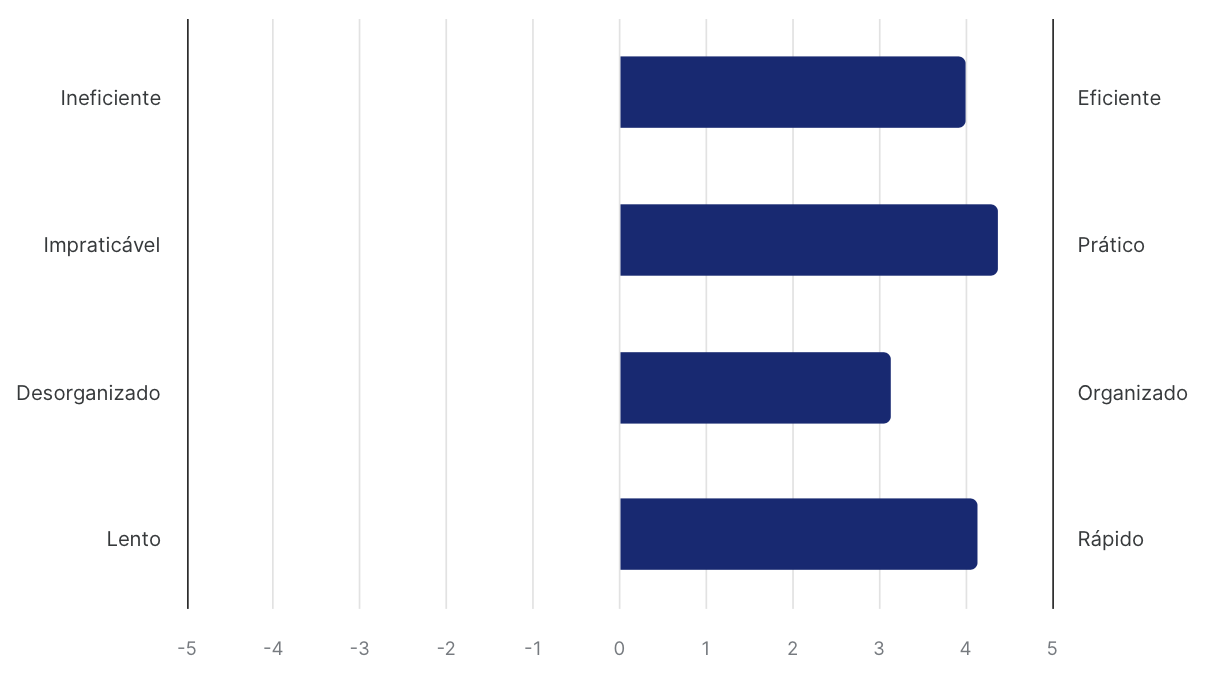
\includegraphics[scale=0.4]{figuras/resultados/ux-5.png}
    \label{fig:ux-5}
    \legend{Fonte: Eonay e Klenilmar (2024).}
\end{figure}

Alguns comentários deixados sobre eficiência na avaliação:
\begin{citacao}

\item "Funcionou no internet explorer sem precisar de login é melhor ainda";
\item "A ferramenta informa quando falta algum campo para preencher";
\item "A entrega dos resultados é rápida e eficiente".

\end{citacao}

Essa eficiência do software é amplamente discutida na engenharia de software por conta das inúmeras variáveis que influenciam neste processo que, neste caro, ocorre geograficamente distante de cada usuário que utiliza e se mantém eficiente, para \citeonline{smith2022software}:

\begin{citacao}
A eficiência do software é um atributo crítico que impacta diretamente o desempenho dos sistemas e a satisfação dos usuários. Programas otimizados reduzem o consumo de recursos computacionais, como tempo de processamento e memória, o que é essencial em sistemas de grande escala ou ambientes com recursos limitados. Além disso, a eficiência contribui para maior sustentabilidade ao minimizar a demanda energética associada ao uso prolongado de dispositivos computacionais.

Adotar práticas de engenharia de software voltadas à eficiência requer uma abordagem multidimensional, combinando design cuidadoso, escolha criteriosa de algoritmos e técnicas de otimização em níveis de código e sistema. Estudos mostram que, embora a busca por eficiência possa aumentar a complexidade inicial do desenvolvimento, ela resulta em benefícios significativos durante a operação e manutenção do software.
\end{citacao}

Todas as características avaliadas anteriormente auxiliam na motivação dos participantes em utilizar, Figura \ref{fig:ux-7}, se tornando motivante e interessante por uma ou mais características excitantes, motivador do apreço ou desapreço ao software.

\begin{figure}[h!]
    \caption{Você se sente motivado a utilizar o produto novamente}
    \centering
    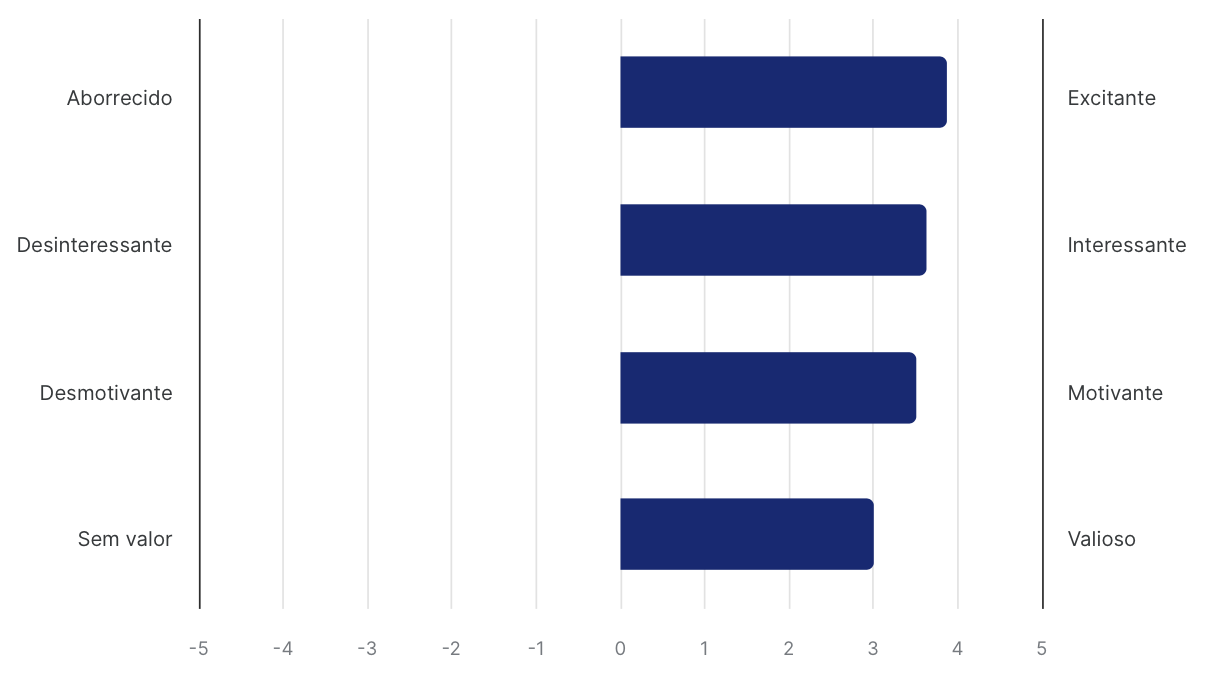
\includegraphics[scale=0.4]{figuras/resultados/ux-7.png}
    \label{fig:ux-7}
    \legend{Fonte: Eonay e Klenilmar (2024).}
\end{figure}


Alguns comentários deixados sobre estimulação na avaliação:
\begin{citacao}
\item "Tem que colocar as outras propriedades que as matrizes possuem";
\item "O Mathix tem potencial de estimular a continuidade do uso da ferramenta, pois habilita a curiosidade de testar cada uma das propriedades/funções disponíveis e de saber como se chegou ao resultado".
\end{citacao}


O uso dessas tecnologias democratiza o acesso a experiências que, de outra forma, poderiam ser limitadas por recursos financeiros ou geográficos. Produtos Educacionais com estimulação de software oferecem oportunidades iguais de aprendizado, independentemente do contexto socioeconômico dos alunos. Assim, ao integrar soluções tecnológicas no ensino, instituições de educação contribuem para a formação de profissionais mais capacitados e preparados para enfrentar os desafios do mundo de trabalho, fortalecendo o papel da tecnologia como um catalisador do aprendizado inclusivo e inovador.

A inovação no desenvolvimento de software tem sido um fator fundamental na criação de ferramentas educacionais que buscam aprimorar o processo de ensino e aprendizagem. A introdução de tecnologias como \textbf{inteligência artificial, gamificação e aprendizado adaptativo} tem permitido que as ferramentas educacionais se tornem mais personalizadas, interativas e eficazes no atendimento das necessidades individuais dos estudantes. Essas inovações possibilitam um ambiente mais dinâmico e atraente, favorecendo a participação ativa e o engajamento dos alunos \cite{santos2022inovacao}. Figura \ref{fig:ux-9} mostra a avaliação no quesito inovação.

\begin{figure}[h!]
    \caption{O produto é inovador e criativo}
    \centering
    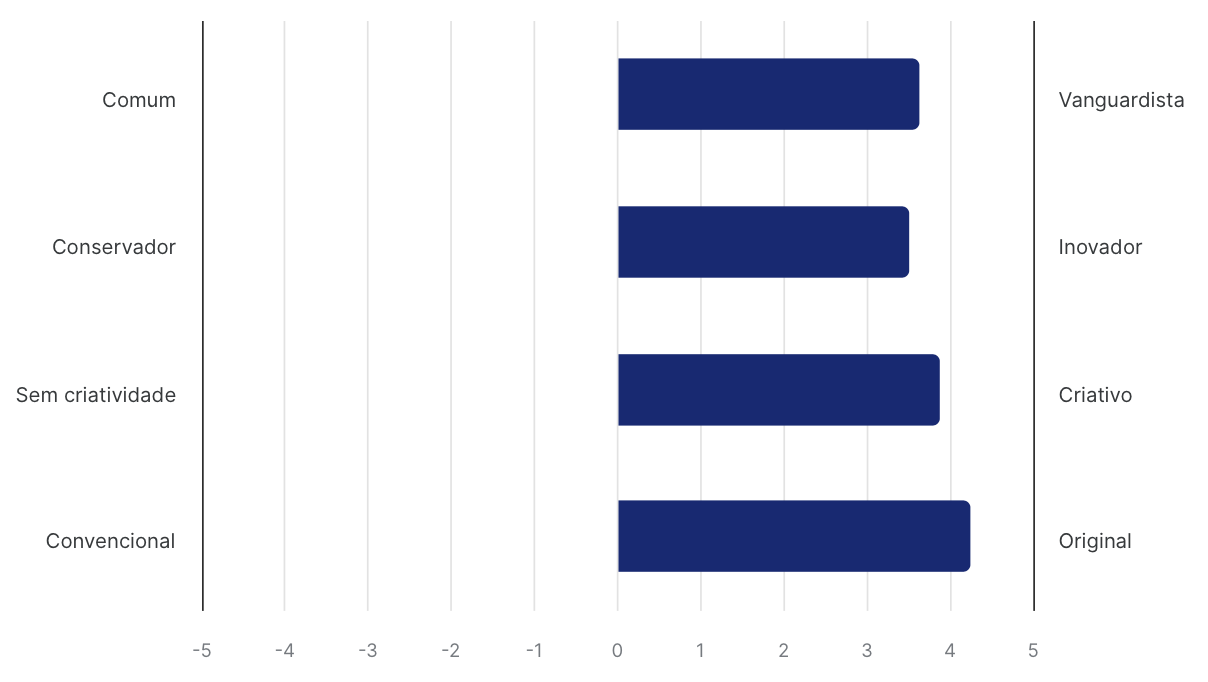
\includegraphics[scale=0.4]{figuras/resultados/ux-9.png}
    \label{fig:ux-9}
    \legend{Fonte: Eonay e Klenilmar (2024).}
\end{figure}

Alguns comentários deixados sobre novidade na avaliação:
\begin{citacao}
\item "Para utilizar matrizes no computador apenas conhecia o matlab que é bem mais completo";
\item "Eu achei inovador, não vejo tantas opções disponíveis de ferramentas com enfoque no assunto matemático explorado pelo Mathix, a maioria é sempre na categoria jogos digitais".
\end{citacao}

A compreensão é fundamental para para a perspicuidade do Mathix como plataforma e de fácil familiaridade principalmente pela questão da interface, Figura \ref{fig:ux-11} traz os resultados da analise sobre a familiaridade e compreensão da proposta.


\begin{figure}[h!]
    \caption{O produto é fácil de entender e de se familiarizar}
    \centering
    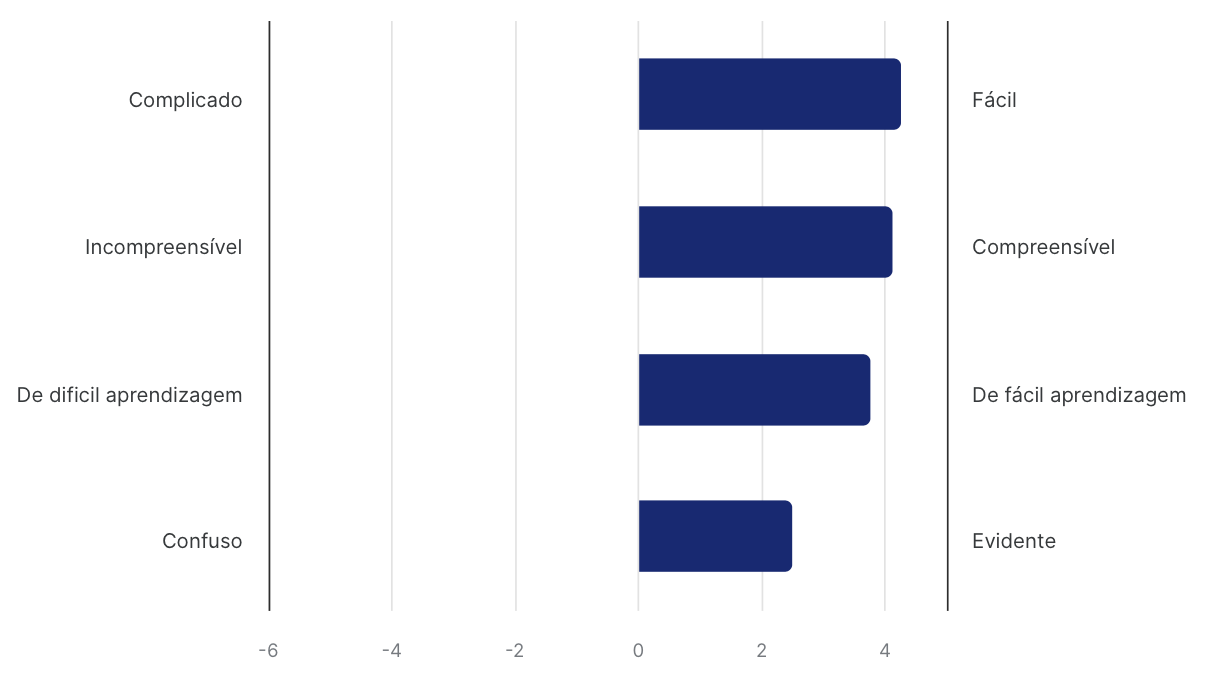
\includegraphics[scale=0.4]{figuras/resultados/ux-11.png}
    \label{fig:ux-11}
    \legend{Fonte: Eonay e Klenilmar (2024).}
\end{figure}

Alguns comentários deixados sobre perspicuidade na avaliação:

\begin{citacao}
\item "Bem direto no que se propõem, pode se tornar melhor com mais recursos";
\item "Achei o produto claro e fácil de entender. Apenas identifiquei que: Se o usuário deixar os campos linhas e colunas vazios não é exibida a mensagem de aviso de que precisa preencher. O usuário consegue digitar o intervalo inicial e intervalo final, ainda que tenha selecionado Valor 0 (zero) ou Valor 1 (um)".
\end{citacao}




De forma geral a avaliação de 1 a 10 para a experiencia do usuário em utilizar o produto educacional na Figura \ref{fig:ux-13}, representado na escala radial que demonstra um alto índice de satisfação no intervalo entre 7 a 10 como resultado indicador de aceitação pelos participantes.

\begin{figure}[h!]
    \caption{Grau de Satisfação do PE (UX)}
    \centering
    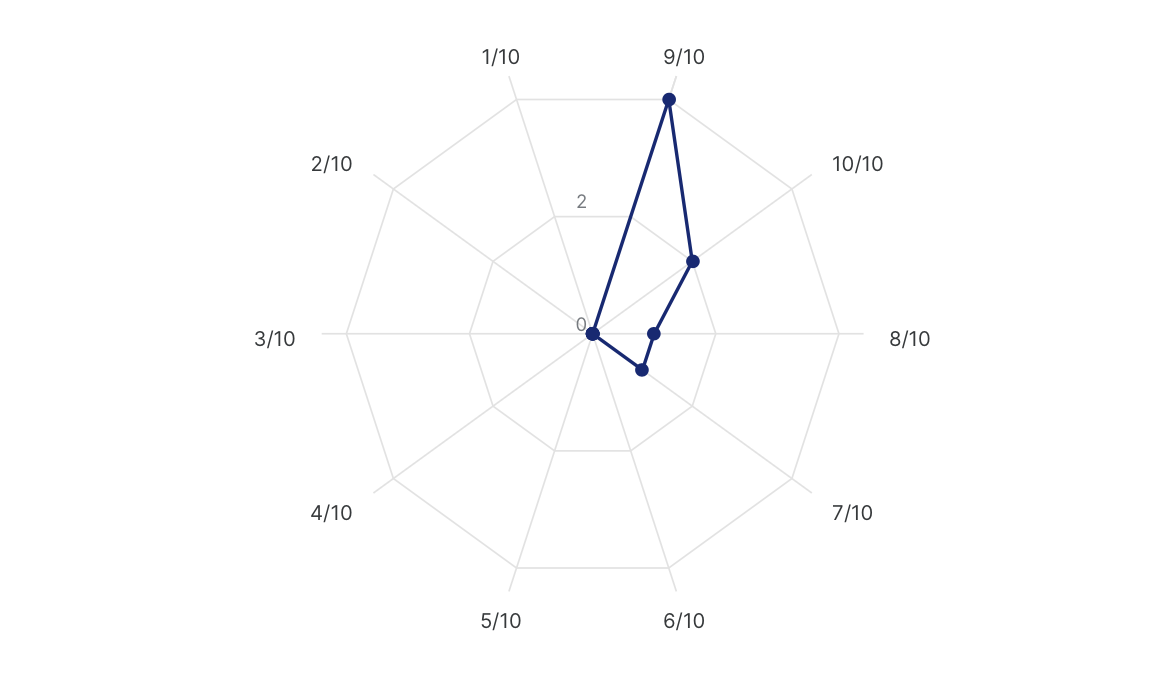
\includegraphics[scale=0.5]{figuras/resultados/satisfacao_ux.png}
    \label{fig:ux-13}
    \legend{Fonte: Eonay e Klenilmar (2024).}
\end{figure}



Por fim de forma optativa fui questionado aos participantes uma avaliação final como pergunta aberta e, obtivemos os \textit{feedbacks}:

\begin{citacao}
    \item "O fato de poder usar via qualquer tipo de dispositivo e de forma gratuita vale a pena";
    \item "Achei fácil de usar e de compreender os resultados".
\end{citacao}













\section{Modelo Acadêmico em LaTeX para ProfEPT IFAP}
\label{model_latex}

O \textbf{LaTeX} é um sistema de preparação de documentos amplamente utilizado em ambientes acadêmicos e científicos, especialmente em áreas que demandam escrita técnica ou matemática. Se baseado na linguagem de marcação \textbf{TeX} e permite criar documentos com alta qualidade tipográfica. O LaTeX é amplamente usado para elaborar artigos, dissertações, teses, e outros tipos de documentos acadêmicos devido à sua precisão e flexibilidade.

Concluir um projeto educacional que envolve a criação de um modelo de documento no formato LaTeX \footnote{https://github.com/eonay/profept-latex}, ajustado às normas da ABNT, é um marco significativo no desenvolvimento de ferramentas para auxiliar acadêmicos e estudantes. Esse tipo de produto educacional não apenas resolve desafios relacionados à padronização, mas também democratiza o acesso a soluções que tornam o processo de escrita científica mais ágil e eficiente. Ao integrar as exigências formais com a praticidade do LaTeX, o modelo se consolida como uma alternativa moderna e poderosa para trabalhos acadêmicos.

O desenvolvimento do modelo LaTeX para ProfEPT com conformidade às normas da ABNT requer uma abordagem meticulosa. Cada detalhe, desde a estrutura básica dos capítulos e sessões até elementos como margens, referências e formatação de citações, precisa ser rigorosamente ajustado. Essa atenção ao detalhe garante que os utilizadores do modelo possam se concentrar no conteúdo, confiando que o formato estará em conformidade com os padrões exigidos pelas instituições e revistas científicas. Assim, o produto educacional não apenas facilita o cumprimento das normas, mas também contribui para a valorização da escrita acadêmica formal.

Além de sua aplicabilidade técnica, o modelo tem potencial pedagógico, pois ajuda estudantes a compreender melhor as diretrizes da ABNT ao utilizá-lo. Como um guia prático, ele funciona como uma ferramenta de aprendizado integrada, permitindo que os usuários vejam na prática como aplicar as regras de formatação, citações e referências. Essa característica transforma o modelo em um recurso valioso para professores e alunos, reforçando a importância da padronização na comunicação científica e promovendo o profissionalismo nos trabalhos apresentados.

A implementação do LaTeX como tecnologia de base adiciona uma camada de relevância ao projeto, pois incentiva a adoção de \textbf{ferramentas computacionais} avançadas no ambiente acadêmico. Apesar de ter uma curva inicial de aprendizado, o LaTeX oferece vantagens significativas, como \textbf{consistência e flexibilidade no design de documentos}. O modelo, ao simplificar a configuração inicial e automatizar aspectos técnicos, torna essa tecnologia mais acessível, especialmente para iniciantes, diminuindo barreiras e estimulando o uso de \textbf{práticas inovadoras no âmbito educacional}.

Por fim, a conclusão desse produto representa uma síntese do esforço \textbf{técnico e educacional}. Ele não apenas resolve problemas práticos enfrentados por acadêmicos, mas também fomenta uma cultura de excelência na produção científica e tecnológica. O impacto positivo de um modelo LaTeX com ajustes às normas da ABNT vai além de facilitar a conformidade normativa, ele promove a integração de tecnologias modernas com a educação, transformando o processo de criação acadêmica em algo mais \textbf{eficiente e acessível} a todos.








